\documentclass[a4paper,11pt]{article}

\usepackage{endnotes}
\let\footnote=\endnote
\usepackage{url,graphicx,array,authblk}
\usepackage[usenames,dvipsnames]{color}

\usepackage{graphicx}
\usepackage[nodisplayskipstretch]{setspace}


\usepackage[margin=1in]{geometry}
\usepackage[utf8]{inputenc}
\usepackage{multirow}
\usepackage{natbib}
\usepackage{amsmath,amssymb,mathtools,amsthm,bbm}
\DeclarePairedDelimiter{\ceil}{\lceil}{\rceil}
\DeclarePairedDelimiter{\floor}{\lfloor}{\rfloor}
\usepackage[title]{appendix}
\newcommand{\HRule}{\rule{\linewidth}{0.35mm}}

\makeatletter

\makeatother
\usepackage{breqn,comment}
\usepackage{booktabs}

\usepackage{subcaption}
\newcommand{\bx}{\mathcal B}
\newcommand{\sx}{\mathcal S}
\newcommand{\MSHAT}{m^\sx}
\newcommand{\MBHAT}{m^{\bx}}
\newcommand{\MBX}{\frac{m^\bx}{1-m^\bx}}
\newcommand{\DNULL}{\frac{\alpha m^{\sx}i^{\bx}-\left(1-\alpha\right)\frac{m^{\bx}}{1-m^{\bx}}i^{\sx}}{i^{\bx}i^{\sx}}}
\newcommand{\DSCF}{\frac{\alpha i^{\sx}+\left(1-\alpha\right)i^{RF}}{i^{RF}}d^{0^*}}

\newcommand{\BA}{\alpha}
\newcommand{\SA}{{1-\alpha}}

\newcommand{\mm}{\mu}
\newcommand{\vv}{\nu}
\newcommand{\ISS}{i^{\sx,0}}
\newcommand{\ISR}{i^{\sx,0}+r}
\newcommand{\IBR}{i^{\bx,0}+r}
\newcommand{\IS}{i^{\sx}}
\newcommand{\IB}{i^{\bx}}
\newcommand{\ISCFR}{i^{RF,0}+r}
\newcommand{\ISRP}{\left(\ISR\right)}
\newcommand{\IBRP}{\left(\IBR\right)}
\newcommand{\ISCFRP}{\left(\ISCFR\right)}
\newcommand{\cites}[1]{\citeauthor{#1}'s (\citeyear{#1})}
\newcommand{\dref}{\widehat d}
\newcommand{\equalD}{\overset{!}{=}}

%\DeclareMathOperator*{\argmax}{arg\,max}
%\DeclareMathOperator*{\argmin}{arg\,min}

\usepackage{placeins}

\usepackage{listings}
\usepackage{float,mdwlist,enumitem}
\usepackage{footmisc}

\newcolumntype{C}[1]{>{\centering\arraybackslash}p{#1}} 
\newcolumntype{L}[1]{>{\raggedright\arraybackslash}p{#1}} 
\newcolumntype{R}[1]{>{\raggedleft\arraybackslash}p{#1}} 
\newlength\interColSepSmall
\newlength\interColSepLarge
\setlength{\interColSepSmall}{0.2em}
\setlength{\interColSepLarge}{0.4em}

%\usepackage{etex}

\newcommand{\PValue}[1]{($p<#1$)}
\newcommand{\Ex}{\mathbb{E}}
\newcommand{\rf}{\mathrm{rf}}
\newcommand{\dHyp}{d^h_r}
\renewcommand{\~}[1]{\tilde{#1}}
\renewcommand{\-}[1]{\overline{#1}}
\newcommand{\D}[0]{\ensuremath{\mathrm{d}}}
\newcommand{\pDefSig}[0]{${}^{+} p< 0.10$,${}^{*} p <0.05$,${}^{**} p <0.01$,${}^{***} p <0.001$}
%\newcommand{\pDefSig}[0]{${}^{*}\mathrm p <0.05$,${}^{**}\mathrm p <0.01$,${}^{***}\mathrm p <0.001$}
\newcommand{\pDefSigCor}[0]{${}^{*} p <0.05$}
\DeclareMathOperator*{\argmax}{arg\,max}
\DeclareMathOperator*{\argmin}{arg\,min}
\usepackage{array}
\usepackage{makecell}

\renewcommand\theadalign{cb}
\renewcommand\theadfont{\bfseries}
\renewcommand\theadgape{\Gape[4pt]}
\renewcommand\cellgape{\Gape[4pt]}

\setlength{\parindent}{0em}
\setlength{\parskip}{0.4em}

\usepackage{xurl}
\usepackage[colorlinks = true,
            linkcolor =black,
            urlcolor  = black,
            citecolor = black,
            anchorcolor = black]{hyperref}


\usepackage{siunitx,enumitem}
\usepackage{dcolumn}
%\newcolumntype{d}[1]{D{.}{.}{#1}}
\newcommand{\muc}[2]{\multicolumn{1}{C{#1}}{#2}}
\newcommand{\suc}[1]{\multicolumn{1}{c}{#1}}

\newtheorem{hypothesis}{Hypothesis}
\newtheorem{definition}{Definition}
\newtheorem{proposition}{Proposition}
\newtheorem{corollary}{Corollary}

%\usepackage{booktabs}
\usepackage{siunitx}
\newcolumntype{d}{S[input-symbols = ()]}

% Natbib setup for author-year style
\usepackage{natbib}
 \bibpunct[, ]{(}{)}{,}{a}{}{,}%
 \def\bibfont{\small}%
 \def\bibsep{\smallskipamount}%
 \def\bibhang{24pt}%
 \def\newblock{\ }%
 \def\BIBand{and}%

  \usepackage{titlesec}
%\newcommand{\subsubsubsection}[1]{\paragraph{#1}$\;$\vspace{-2pt}\\}
\newcommand{\subsubsubsection}[1]{\paragraph{#1}$\;$\vspace{-2pt}\\}
\titleformat{\subsubsubsection}
{\normalfont\normalsize\bfseries}{\thesubsubsubsection}{-1em}{}
\titlespacing*{\subsubsubsection}
{0pt}{-3ex plus -1ex minus 1.2ex}{-3.5ex plus .02ex}

\expandafter\def\expandafter\normalsize\expandafter{%
    \normalsize%
    \setlength\abovedisplayskip{5pt}%
    \setlength\belowdisplayskip{3pt}%
    \setlength\abovedisplayshortskip{0pt}%
    \setlength\belowdisplayshortskip{2pt}%
}

\newcommand{\Hypo}[2]{\begin{hypothesis}\label{hypo:#1}#2\end{hypothesis}}
\newcommand{\killSpace}{$\;$\vspace{-36pt}\\}
\setlength{\abovecaptionskip}{-1pt}
\setlength{\belowcaptionskip}{-7pt}
\setlength{\parindent}{0pt}
\setlength{\parskip}{6pt}
\titlespacing*{\section}
{0pt}{0.0ex plus 0ex minus .9ex}{-1.2ex plus .01ex}
\titlespacing*{\subsection}
{0pt}{0.0ex plus 0ex minus .9ex}{-1.2ex plus .01ex}
\titlespacing*{\subsubsection}
{0pt}{0.0ex plus 0ex minus .9ex}{0.1ex plus .1ex}

\makeatletter
\def\thm@space@setup{\thm@preskip=0pt
\thm@postskip=0pt}
\makeatother

\usepackage{chngcntr}
\newcounter{pretheorem}
\counterwithin{hypothesis}{pretheorem}

\renewcommand\thehypothesis{\arabic{pretheorem}\alph{hypothesis}}
\newcommand{\theoremgroup}{\refstepcounter{pretheorem}}


\title{Empirical Evidence about Payment Term Extensions\\ in the Reverse Factoring Context}
\date{}
%\author{(blinded for peer-review)\vspace{-24pt}}
\author[1]{David Wuttke}
\affil[1]{Technische Universit\"at M\"unchen, TUM School of Management, TUM Campus Heilbronn, Bildungscampus 9, 74076 Heilbronn, Germany, david.wuttke@tum.de\vspace{-36pt}}


%%%%%%%%%%%%%%%%
\begin{document}
%%%%%%%%%%%%%%%%
\maketitle%

\vspace{6pt}
%\AFF{} %, \URL{}}
%k
\noindent%
\textbf{Abstract:} Reverse factoring (RF) is a highly relevant form of supply chain finance. Whereas extant analytical studies indicate how RF should enable buyers to extend payment terms with existing suppliers, sufficient empirical evidence is lacking. To hypothesize on payment term extensions, we study three motives---financing cost, fairness, and standardization. Our empirical evidence indicates the presence of fairness concerns and standardization of payment terms. However, it suggests financing costs play a more minor role than expected. Managers should thus be prudent in applying simple formulas to estimate benefits inherent to RF; they seem fairly inconsistent with industry practice. Harmonizing payment terms, instead, is more common.\vspace{3pt}
%

% Sample
%\KEYWORDS{deterministic inventory theory; infinite linear programming duality;
%  existence of optimal policies; semi-Markov decision process; cyclic schedule}
\noindent%
\textbf{Keywords:} reverse factoring; supply chain finance; econometrics; hypotheses testing

%\HISTORY{}
\doublespacing

%%%%%%%%%%%%%%%%%%%%%%%%%%%%%%%%%%%%%%%%%%%%%%%%%%%%%%%%%%%%%%%%%%%%%%

% Samples of sectioning (and labeling) in MNSC
% NOTE: (1) \section and \subsection do NOT end with a period
%       (2) \subsubsection and lower need end punctuation
%       (3) capitalization is as shown (title style).
%
%\section{Introduction.}\label{intro} %%1.
%\subsection{Duality and the Classical EOQ Problem.}\label{class-EOQ} %% 1.1.
%\subsection{Outline.}\label{outline1} %% 1.2.
%\subsubsection{Cyclic Schedules for the General Deterministic SMDP.}
%  \label{cyclic-schedules} %% 1.2.1
%\section{Problem Description.}\label{problemdescription} %% 2.

\section{Introduction}

%\begin{itemize}
%    \item write up proofs
%    \item interviews\footnote{https://www.crxmarkets.com/crx-marketplace/for-%corporates/calculator/}\footnote{https://www.citibank.com/tts/sa/supplier-finance/ge/index.jsp}
%    \item All motivation and interview stuff goes to the introduction.
%    \item remove adjectives, simplify and shorten
%\end{itemize}

Even buying firms with solid credit ratings turn to their supply chain to reduce their financing costs and improve their working capital \citep{Filbeck2016}. They pay their suppliers according to long payment terms \citep{Hu2018}, such as when Boeing increased its payment terms to 120 days, as opposed to 30 days \citep{Scott2016}, and Anheuser Busch InBev strived for payment terms of 120 days \citep{Daneshkhu2015}. Procter \& Gamble demanded its suppliers to wait 75 days until getting paid, resulting in increases of about \$1 billion in its cash flows \citep{Strom2015}. Suppliers in weaker bargaining positions often feel more compelled to accept the longest payment terms, whereas more powerful suppliers get paid faster \citep{Fabbri2016}. However, putting financial pressure on weaker suppliers increases their economic risk \citep{Boissay2007}.

To extend payment terms with all suppliers without jeopardizing the liquidity of the upstream supply chain, many large buying firms have adopted reverse factoring (RF) \citep{Herath2015,vanderVliet2015, Wuttke2019}. With a potential market volume of \$20 billion \citep{Herath2015} and a quickly growing number of significant firms using RF (e.g., Walmart\footnote{\url{https://www.blendedfinance.earth/supply-chain-innovations/2020/11/16/walmarts-supply-chain-financing-programme}, accessed on 08/23/2023.}%, %Siemens\footnote{\url{https://new.siemens.com/global/en/company/about/corporate-functions/supply-chain-management/collaborating-with-siemens/supply-chain-finance.html}, accessed on 08/23/2023.}, 
and Michelin\footnote{\url{https://primerevenue.com/resources/news/michelin-recognized-for-highly-effective-supply-chain-finance-implementation/}, accessed on 08/23/2023.}), RF is among the most important supply chain finance arrangements. RF always involves a buying firm, a supplier, and an RF provider (which may be a bank). After the buying firm's invoice approval, the RF provider immediately pays suppliers in the RF program. The suppliers receive the total invoice amount minus an RF interest charge. This charge depends on the payment term (the longer the payment term, the higher the cost), as well as on the buying firm's usually strong credit rating, such that it tends to be substantially cheaper for the suppliers compared to other sources of financing (otherwise, they typically would not use RF). After the payment term, the buying firm pays the RF provider the total invoice amount. Suppliers thus benefit from reduced financing costs, paying their buyer's interest rate instead of their own. So, buyers can use RF to extend payment terms without sacrificing their upstream supply chain's liquidity. But the question arises: how much can they extend payment terms for each supplier? Would it be worth the effort required to adopt RF?

% This mechanism, the impact of RF on performance, and operational decisions are core to ample analytical studies \citep{Hu2018, Kouvelis2020, Lekkakos2016, Tanrisever2012,vanderVliet2015, Wuttke2016}. Whereas they do not primarily seek to predict actual payment term extensions in industry, such predictions would be helpful for supply chain managers interested in RF to estimate the potential benefits and craft an optimal payment term strategy.

To predict payment term extensions, they must likely account for more than just the interest rate difference. Discussions with and publications by RF providers indicate some potentially relevant motives. CRX Markets and Citibank, for instance, emphasize \textit{financing costs} by offering online calculators.\footnote{\url{https://www.crxmarkets.com/crx-marketplace/for-corporates/calculator} and \url{https://www.citibank.com/tts/sa/supplier-finance/ge/index.jsp}, accessed on 08/23/2023.} With their online tools, managers can enter the current conditions (payment terms and interest rates) and the RF conditions (new payment terms and RF interest rate) and calculate the supplier's savings. This is meant to indicate the considerable potential to extend payment terms. In addition, PrimeRevenue emphasizes \textit{fairness} concerns,\footnote{\url{https://primerevenue.com/resources/blog/fair}, accessed on 08/23/2023.} picking up on the criticism that RF helps powerful buyers to extend payment terms unduly \citep{Pettypiece2015}. This fintech emphasizes that managers also account for whether they perceive an agreement as fair. Or consider Orbian, whose chairman recently emphasized the potential of \textit{standardizing} payment terms with RF.\footnote{\url{https://orbian.com/using-carrots-and-sticks-to-sustain-supply-chain-finance/}, accessed on 08/23/2023.} Buyers that standardize payment terms reduce the differentiation among their suppliers \citep{Peura2017}, they can reduce the administrative effort required for managing different terms, and reduce errors resulting from a lack of standardization. Do all three motives--- financing cost, fairness, and standardization---affect payment term extensions? Or is the financing cost motive dominant in industry? After all, the primary motivation for adopting RF is to extend payment terms \citep{Liebl2016, Wuttke2013}. In addition, the financing cost motive is most central to extant analytical studies on RF \citep{Hu2018, Kouvelis2020, Lekkakos2016, Tanrisever2012,vanderVliet2015, Wuttke2016}. In contrast, neither fairness nor standardization motives have received the same academic attention in the context of RF adoption \citep[with the exception][]{banerjee2021}. Put differently, how much should managers rely on RF providers' statements on fairness and standardization? Do they really play a role?

To provide answers, we derive a Nash bargaining model with financing cost, fairness, and standardization motives. Building on our analytical results, we derive six hypotheses and 
 test those on a dataset of $N=1,898$ buyer-supplier dyads. Contradicting our intuition that the financing cost motive is likely dominant, we find mainly support for the fairness and the standardization motives, whereas the financing cost motive is less salient. Therefore, our findings change the perspective that we should take on RF. Parsing the results of our study carefully, managers of buying firms seem not to adopt RF to maximize their payment terms according to strategies implied by online calculators and simple formulas. Instead, they remove their suppliers' differences in initial payment terms, creating more equality and homogeneity. This harmonization effect suggests that the hitherto understudied motives of fairness and standardization are essential, opening the avenue for analytical and empirical researchers.% Whereas many studies test game-theoretical predictions through experiments \citep{Katok2009, Croson2013, donohue2016}, we add to a relatively limited set of studies that test game-theoretical predictions with secondary data \citep{Sluis2016, Tunca2017}, responding to the call for more intertwinement among research methods \citep{Singhal2012}.

\section{Related literature}\label{sec:literature}
The finance and operations interface is receiving increasing attention \citep{Babich2004,Kouvelis2012,Zhao2015}. Many studies indicate that cash flow optimization and liquidity management are important objectives complementing profit maximization \citep{Boissay2013, Filbeck2016, Kouvelis2012}. Empirical studies find how firms agree on payment terms without reverse factoring (RF) \citep{Summers2002,Fabbri2016}. Powerful buyers often bargain for long payment terms \citep{Fabbri2016}. By enabling faster cash flows, RF directly affects this decision. 
 
There are several empirical, operations-management-related studies on RF. \citet{Liebl2016} and \citet{Wuttke2013} both derive insights using case studies. \citet{Liebl2016} explores the objectives of, antecedents to, and barriers to RF adoption. They find that buyers mainly adopt RF to extend payment terms and reduce supply chain risks. \citet{Wuttke2013} focus on the adoption process from a buying firm's perspective and find that RF adoption requires a series of organizational and procedural adjustments. \citet{Wuttke2019}, studying the adoption of RF by suppliers, derive and test efficiency and legitimacy motives as drivers. They find that suppliers adopt RF faster if they are small, expect big benefits, and face considerable institutional pressures. However, to the best of our knowledge, no empirical study examines how buyers extend payment terms, and when they extend by more or fewer days. 

Prior analytical studies typically depart from inventory models \citep{Lekkakos2016,Kouvelis2020,Tanrisever2012,vanderVliet2015}, models of financial flexibility \citep{Grueter2017,Hu2018}, or innovation diffusion models \citep{DelloIacono2015, Wuttke2016} in their effort to identify the RF value proposition. Those studies typically characterize the optimal payment term extensions, noting that, in equilibrium, those tend to be positive \citep{Hu2018,Lekkakos2016}. The objective of virtually all game theoretic models of RF is to understand underlying tradeoffs and mechanisms \citep{Grueter2017, Hu2018, Kouvelis2020, Lekkakos2016, Tanrisever2012, vanderVliet2015, Wuttke2016}. Whereas they all provide fascinating insights and often counter-intuitive results (for instance, when \citet{Kouvelis2020} finds that not all buyers should extend payment terms when adopting RF), their purpose is not necessarily to explain actual behavior. So, despite their mathematical rigor, it might be that the empirical setting differs from some assumptions, limiting the scope for predictions. We complement this literature as we provide a parsimonious model seeking to describe actual behavior so that we can test our predictions with data from several RF programs. 

Whereas most studies on RF examine financial aspects, \citet{banerjee2021} examine RF adoption decisions through a choice-based conjoint experimental design. In their experiment, subjects refused RF adoption significantly more often when they perceived unfairness. We also consider fairness but study its impact on a bargaining outcome instead of the adoption decision. We further examine actual decisions in a secondary-data study. More generally, we draw from the literature on fairness concerns in supply chains. The theory on fairness is broad \citep[see][]{Fehr1999}; we relate primarily to those studies that examine how fairness concerns affect decisions in supply chains like \citet{Cui2007}, providing a game-theoretical model of fair-minded supply chain firms, and \citet{Cappelen2007}, examining various fairness ideals in experiments. In our model, we also assume actors to be fair-minded as we model the particular case where neither firm wants to end up below their fairness ideal.

\section{Analytical predictions}\label{sec:model}
We derive analytical predictions on payment term extensions, complementing extant research in three regards. First, to be consistent with empirical studies that examine how firms agree on payment terms \citep{Fabbri2016, Summers2002}, we assume Nash bargaining instead of a Stackelberg game. Second, we introduce the notion of fairness concerns \citep{Cappelen2007, Cui2007,banerjee2021} to bargaining over payment terms in the RF context. Buyers (suppliers) perceive disutility if their new payment terms fall below (exceed) a reference point, such as the industry average. Third, we introduce standardization benefits for the buyer. Those benefits arise when terms become identical as this reduces differentiation among suppliers \citep{Peura2017}, the administrative effort required for managing contracts, and the risks of errors. Since one buyer uses RF with multiple suppliers in an RF program but one supplier uses RF only with this buyer, standardization benefits only arise for buyers.

\subsection{Model}
The status quo is the best alternative to a negotiated agreement. Consider buyer $b$ and supplier~$s$. Before adopting RF, the buyer's payment terms are $d_0$; that is, it pays the supplier the invoice value $d_0$ days after receiving goods and services. Without loss of generality, we normalize the invoice value to one. By paying the supplier after payment terms $d_0$, the buyer can invest the same amount with interest rate $i_b$, leading to utility $U_{b,0}\left(d_0\right)=i_bd_0$. In contrast, the supplier incurs financing costs of interest rate $i_s$ leading to a utility of $U_{s,0}\left(d_0\right)=-i_sd_0$.

Both players bargain over the RF payment terms, $d_r$, when adopting RF. The supplier's RF interest rate is $i_r$. We only consider cases where $i_r< i_s$, so the supply chain is better off adopting RF. We refer to the reduced financing costs as the \textit{financing cost motive}. The \textit{fairness motive} emerges when adopting RF and deciding how to split the difference \citep{banerjee2021}. Following \citet{Cappelen2007}, we assume a fairness ideal in the form of a reference point, $\dref$, such that the buyer perceives marginal disutility of $\beta\geq 0$ for ending up below this reference, and the supplier perceives marginal disutility $\gamma\geq 0$ for ending up above this reference. We capture the third motive, the \textit{standardization motive}, by assuming the buyer obtains extra utility $\lambda$ if the bargained terms equal the reference point, which we denote with indicator function $\mathbbm{1}_{\left\{\dref\,\right\}}\left(d^r\right)$. This leads to utility functions,%
\begin{equation}\label{eq:utilities}
    \begin{aligned}
    U_{b,r}\left(d_r\right) = & \underbrace{i_bd_r}_{\substack{\text{financing}\\\text{motive}}} -\;\, \underbrace{\beta \max\left\{0,\left(\dref-d_r\right)\right\}}_{\text{fairness motive}}  \;\,+\underbrace{\lambda \mathbbm{1}_{\left\{\dref\,\right\}}\left(d^r\right)}_{\text{standardization motive}}\\
    U_{s,r}\left(d_r\right) = & \underbrace{-i_rd_r}_{\substack{\text{financing}\\\text{motive}}} -\;\, \underbrace{\gamma \max\left\{0,\left(d_r-\dref\right)\right\}}_{\text{fairness motive}}
    \end{aligned}
\end{equation}  

To avoid extreme cases, we assume a reasonable reference point with $U_{b,r}\left(\dref\,\right)\geq U_{b,0}\left(d_0\right)$ and  $U_{s,r}\left(\dref\,\right)\geq U_{s,0}\left(d_0\right)$. $\gamma=\beta=\lambda=0$ captures the hypothetical case where only the financing cost motive governs the outcome; we refer to this as the hyper-rational benchmark. $\gamma\rightarrow\infty,\,\beta\rightarrow\infty$ captures the case where the fairness motive is fully dominant and $\lambda\rightarrow\infty$ when the standardization motive is fully dominant. Let $\alpha\in(0,1)$ denote the buyer's bargaining power so that it has full power (i.e., becomes a Stackelberg leader) for $\alpha\rightarrow 1$. Then, the Nash Bargaining solution \citep{Owen2013} posits that both parties agree on payment terms $d^{*}_r$ such that,
\begin{equation}\label{eq:obj}
d^{*}_r \in \argmax_{d_r\geq 0}\left\{
\left(
U_{b,r}\left(d_r\right) - U_{b,0}\left(d_0\right)
\right)^\alpha
\left(
U_{s,r}\left(d_r\right) - U_{s,0}\left(d_0\right)
\right)^{\left(1-\alpha\right)}
\right\}.
\end{equation}

\subsection{Financing cost motive (hyper-rational benchmark)}
To study the impact of the fairness and standardization motives more explicitly, we first provide a hyper-rational benchmark where actors only care about the financing cost motive.%
\begin{proposition}[Hyper-rational benchmark]\label{prop:hyper}\singlespacing
    Suppose $\beta=\gamma=\lambda=0$. Then,
    \begin{equation}
        \dHyp := \left(1+\frac{i_s-i_r}{i_r}\alpha\right)d_0
    \end{equation}
    is the unique bargaining outcome.
\end{proposition}%
%
If only the financing cost motive is present, payment terms under RF thus linearly increase in former payment terms, $d_0$. The extension is $\dHyp - d_0 = \frac{i_s-i_r}{i_r}\alpha d_0$. Since, by assumption, $i_s>i_r$, the extension grows in the initial payment terms. As one might surmise, this effect increases in the buyer's bargaining power, $\alpha$. Figure~\ref{fig:hyper:dr} illustrates the equilibrium outcomes. The horizontal axis displays the initial payment terms, $d_0$. The vertical axis displays RF payment terms, $d_r$. The solid graph (bold line) indicates the equilibrium payment terms, $\dHyp$. This figure shows, for a fixed annual RF interest rate, whether the RF payment terms, in equilibrium, would end up below (dark area) or above the reference, $\dref$ (bright area). Since the equilibrium is independent of $\dref$, the graph is linear in $d_0$. More generally, the result in Proposition~\ref{prop:hyper} helps to predict this for any combination of initial payment terms and annual RF interest rate while fixing the remaining parameters, as seen in Figure~\ref{fig:hyper:equilibria}.

%
\begin{figure}[bh]
     \centering
     \begin{subfigure}[b]{0.47\textwidth}
         \centering
         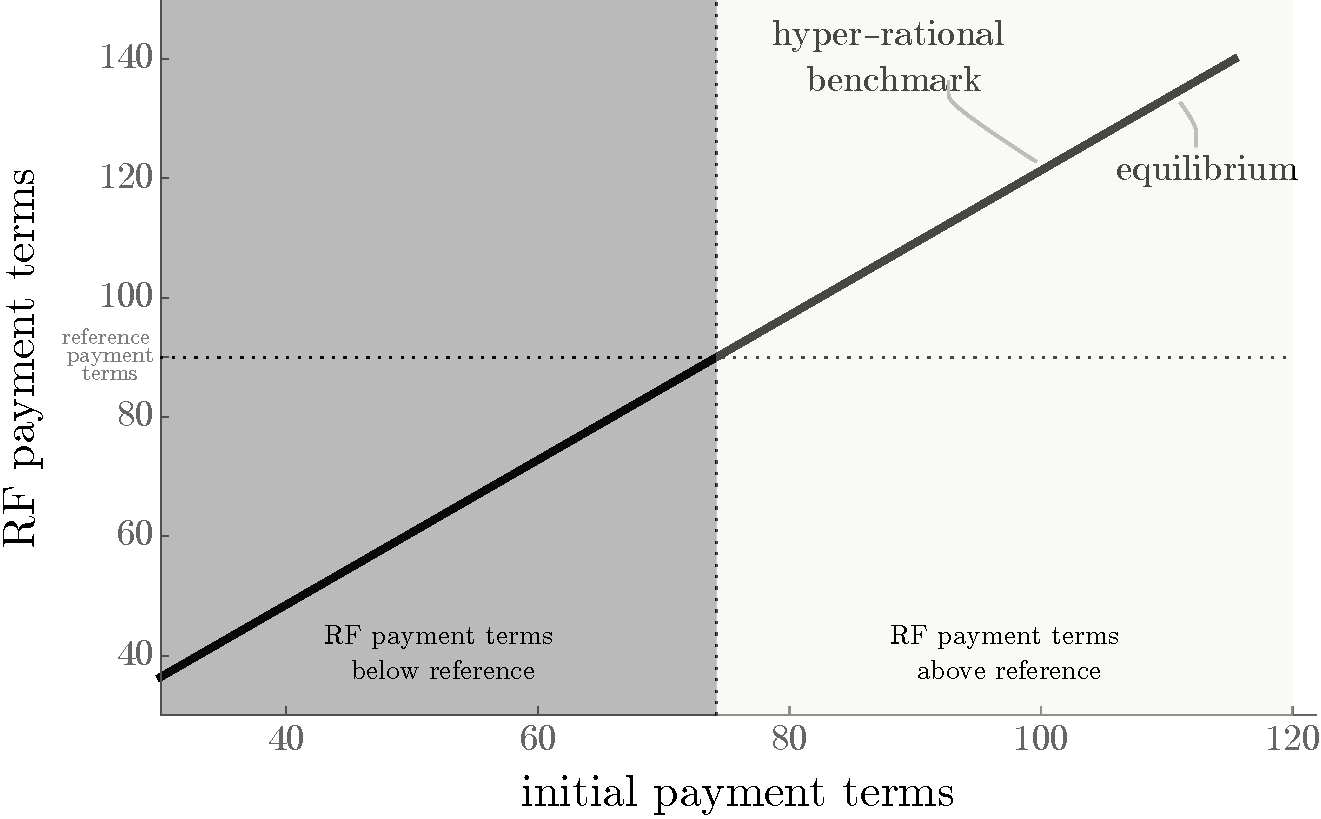
\includegraphics[width=\textwidth]{figures/03_PosteriorTerms_hyperrational_bechmark.pdf}\vspace{7pt}
         \caption{RF payment terms \vspace{12pt}}
         \label{fig:hyper:dr}
     \end{subfigure}
     \hfill
     \begin{subfigure}[b]{0.47\textwidth}
         \centering
         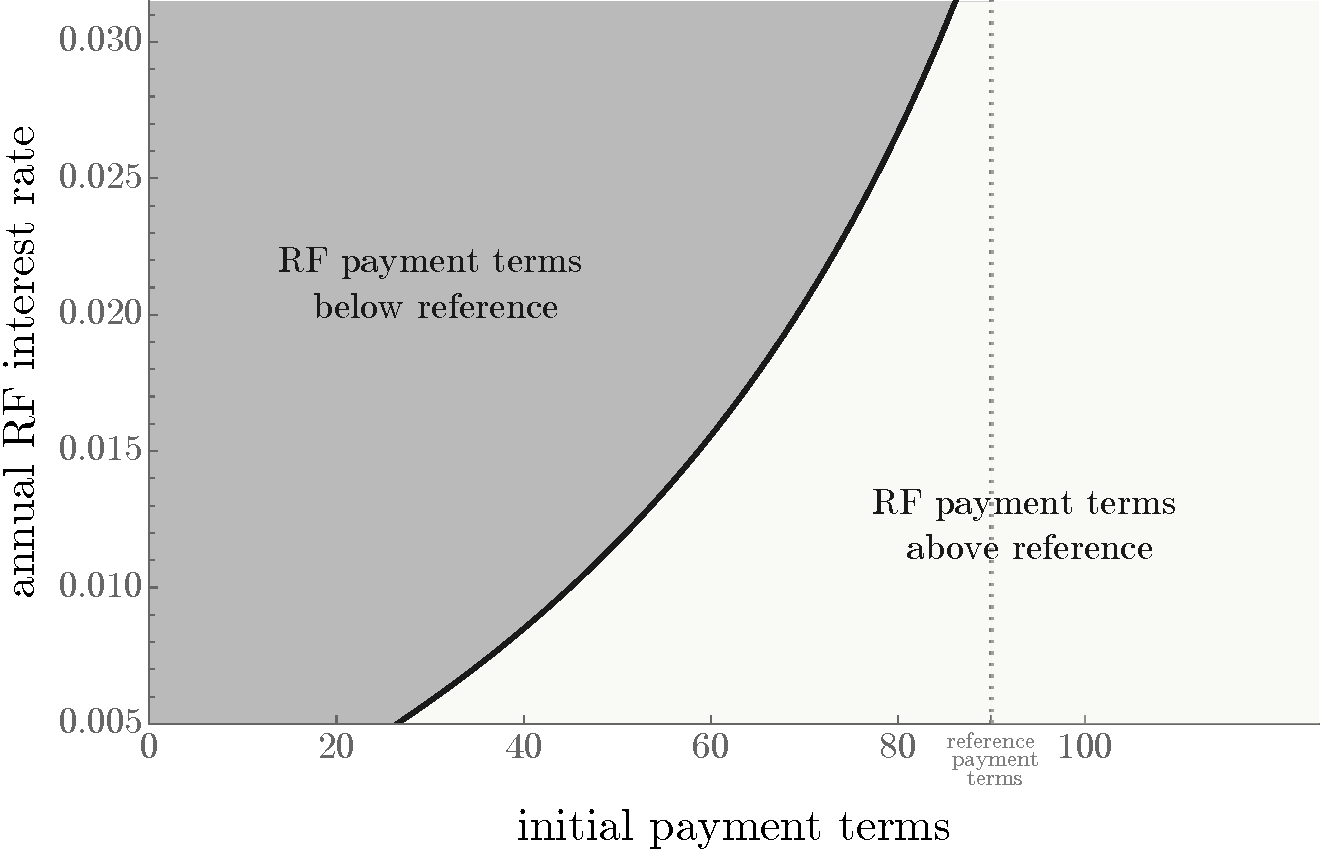
\includegraphics[width=\textwidth]{figures/01_equilibria_hyperrational_benchmark.pdf}
         \caption{RF equilibria\vspace{12pt}}
         \label{fig:hyper:equilibria}
     \end{subfigure}
        \caption{Hyper-rational decision makers}
        \label{fig:hyper}
\end{figure}%
%


\newpage

\subsection{Fairness motive}
Let us focus on the fairness motive by examining $\beta>0$ and $\gamma>0$ while keeping $\lambda=0$.
\begin{proposition}[Fairness motive]\label{prop:fairness}
    Suppose $\beta>0$, $\gamma>0$, and $\lambda=0$. Then,
    \begin{equation}\label{eq:drf}
        d^{f}_r := \begin{cases}
        \dHyp + \frac{(\dref-d_0) (1 - \alpha) \beta}{i_b + \beta}
  & \text{, if } d_0 < \frac{ i_r (i_b + \alpha \beta)}{
  i_b (i_r + \left(i_s- i_r\right) \alpha) + i_s \alpha \beta)}\dref\\
  \dref & \text{, if }d_0\in\left[\frac{ i_r (i_b + \alpha \beta)}{
  i_b (i_r + \left(i_s- i_r\right) \alpha) + i_s \alpha \beta)}\dref,\frac{ i_r + \left(1- \alpha\right) \gamma}{i_r + (i_s-i_r) \alpha + (1-\alpha)\gamma}\dref\right]\\
  \dHyp-\frac{(d_0 i_s-\dref i_r) \alpha \gamma}{i_r (i_r + \gamma)} & \text{, if } d_0 >\frac{ i_r + \left(1- \alpha\right) \gamma}{i_r + (i_s-i_r) \alpha + (1-\alpha)\gamma}\dref
        \end{cases}
    \end{equation}
    is the unique bargaining outcome.
\end{proposition}

This solution features three cases depending on the size of the initial payment terms, $d_0$, relative to the reference value, $\dref$. In the first and third cases, characterized by relatively low and high initial payment terms, respectively, the RF payment terms resemble the hyper-rational benchmark but differ by a function of $\beta$ ($\gamma$) for small (high) initial payment terms. The intermediate range differs structurally: regardless of the initial payment terms, both parties will exactly agree on the reference point, $\dref$. So, even without the standardization motive, the fairness motive can lead to perfect standardization. Intuitively, firms obtain a constant, marginal disutility from deviating from the reference point. The financing cost motive's impact is convex and relatively weak around the reference point: for one firm to gain is for the other to lose. Overall, the fairness motive thus dominates as long as the bargaining outcome is close enough to the reference point. Figure~\ref{fig:fair} illustrates the three cases. %
\begin{figure}[b]
     \centering
     \begin{subfigure}[b]{0.47\textwidth}
         \centering
         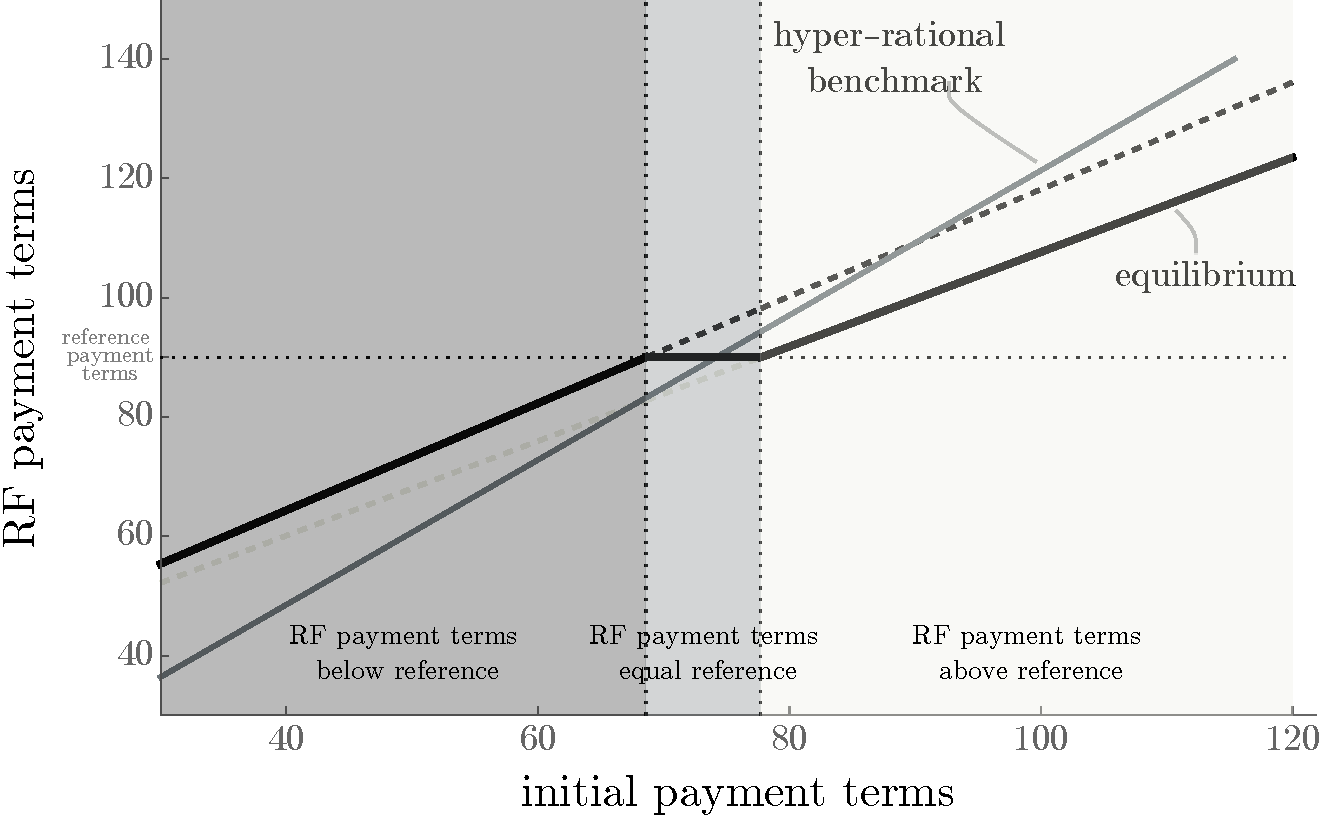
\includegraphics[width=\textwidth]{figures/04_PosteriorTermsFairness.pdf}\vspace{5pt}
         \caption{RF payment terms \vspace{12pt}}
         \label{fig:fair:dr}
     \end{subfigure}
     \hfill
     \begin{subfigure}[b]{0.47\textwidth}
         \centering
         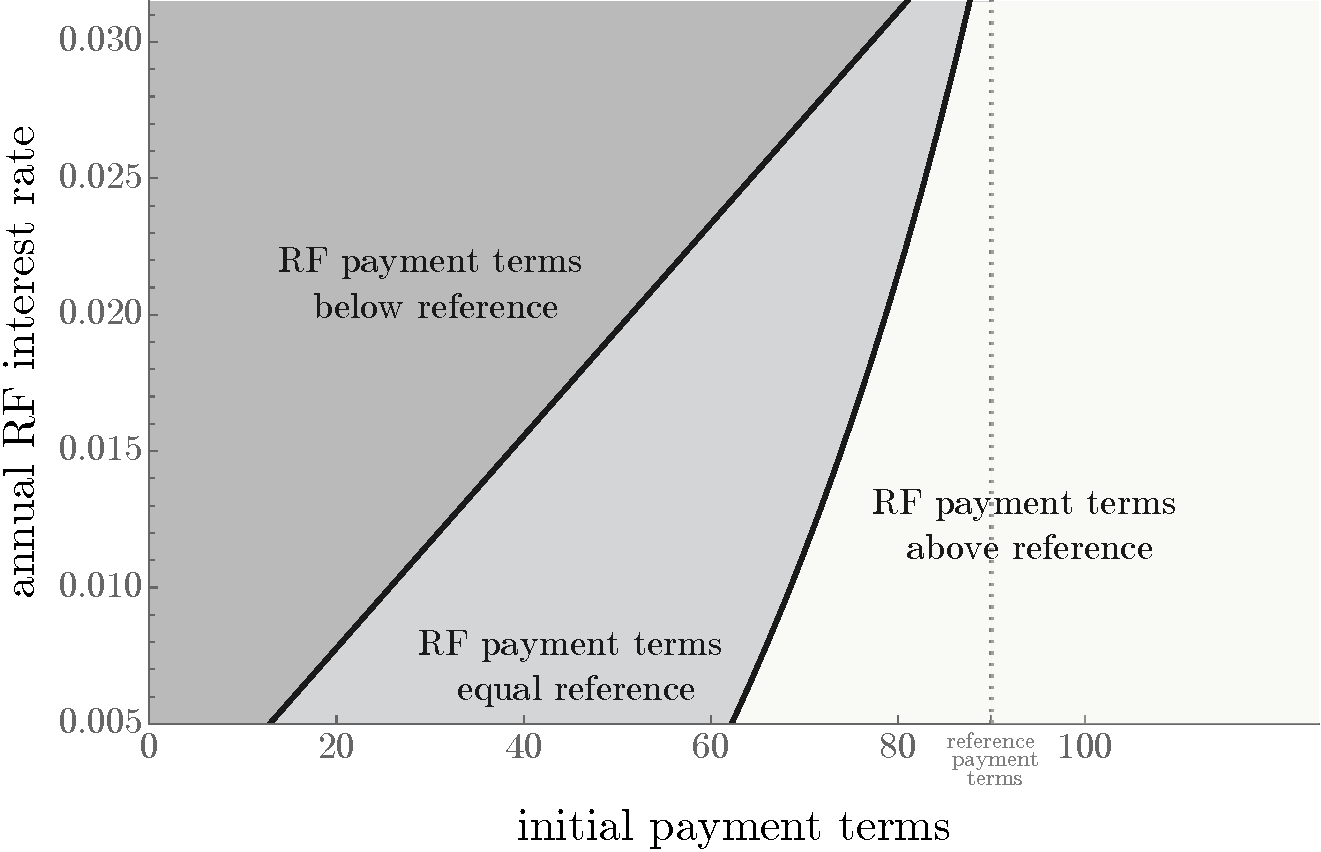
\includegraphics[width=\textwidth]{figures/02_equilibria_fairness.pdf}
         \caption{RF equilibria\vspace{12pt}}
         \label{fig:fair:equilibria}
     \end{subfigure}
        \caption{The fairness motive can lead to standardized payment terms.}
        \label{fig:fair}
\end{figure}%
In Figure~\ref{fig:fair:dr}, perfect standardization occurs for all initial payment terms ranging from about 70 to 78 days, a range that depends on the RF interest rate (Figure~\ref{fig:fair:equilibria}). Figure~\ref{fig:fair:dr} further illustrates that, compared to the hyper-rational benchmark, the fairness motive can lead to larger RF payment terms (below the reference) and smaller RF payment terms (above the reference).

Defining payment term extensions as $d^{f}_r-d_0$, Figure~\ref{fig:delta} displays four scenarios of how initial payment terms inform the equilibrium outcome. Figure~\ref{fig:delta:rational:full} shows the hyper-rational case with a  positive relationship between initial payment terms and extension. Figure~\ref{fig:delta:rational:dominant} features actors with weak fairness motives leading to a similar, yet flatter, slope, but one disrupted by the intermediate range where both agree on $\dref$. In Figure~\ref{fig:delta:fair}, the fairness motives are so strong that the overall effect of initial payment terms is negative. Finally, Figure~\ref{fig:delta:fair:full} displays a scenario where fairness concerns are so dominant that one day more in initial payment terms leads to one day less extension for a broad range of initial payment terms.

\begin{figure}[htb]
      \begin{subfigure}[b]{0.48\textwidth}
         \centering
         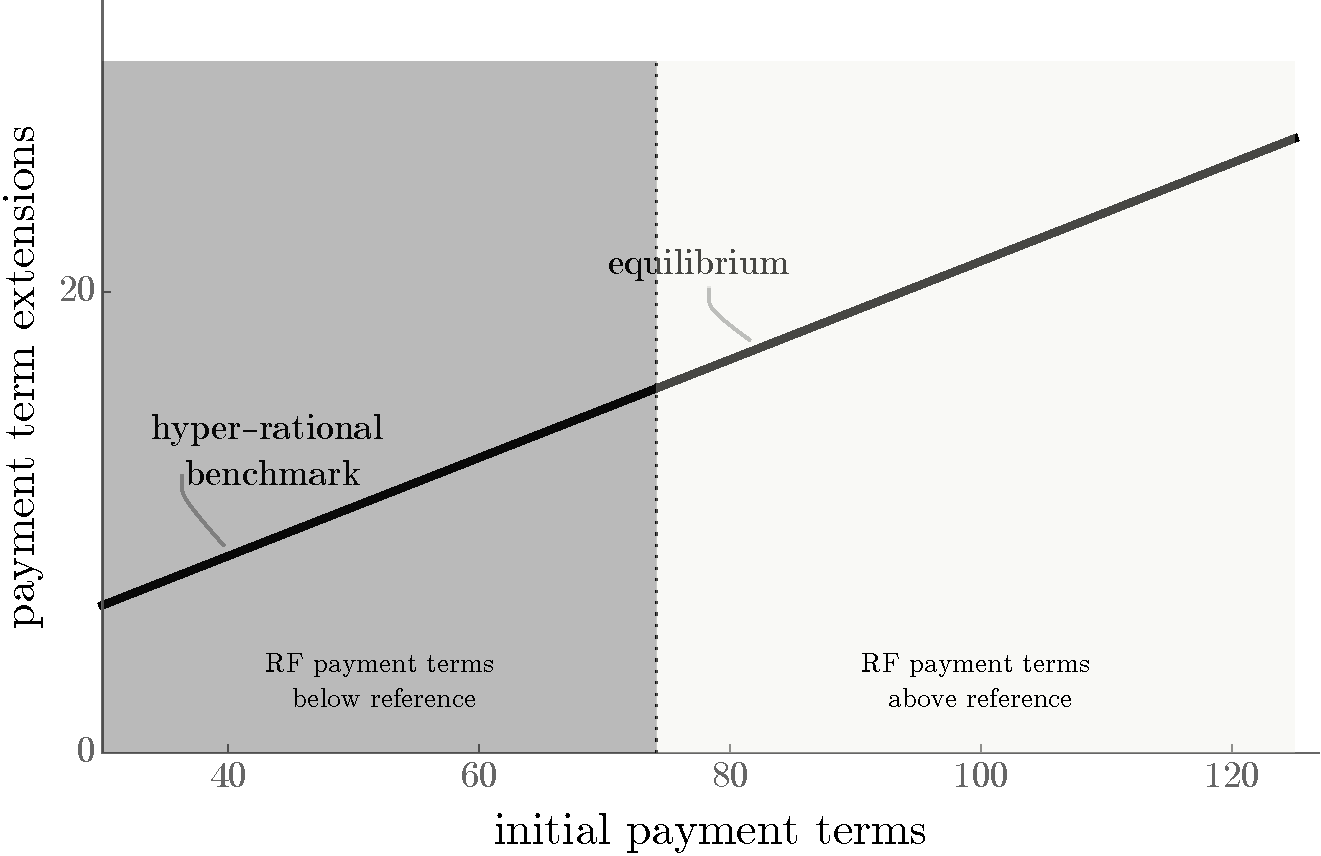
\includegraphics[width=\textwidth]{figures/06_ExtensionFairness_0.pdf}
         \caption{No fairness motive \newline ($\beta=\gamma=0$) \vspace{12pt}}
         \label{fig:delta:rational:full}
     \end{subfigure}\hfill
     \begin{subfigure}[b]{0.48\textwidth}
         \centering
         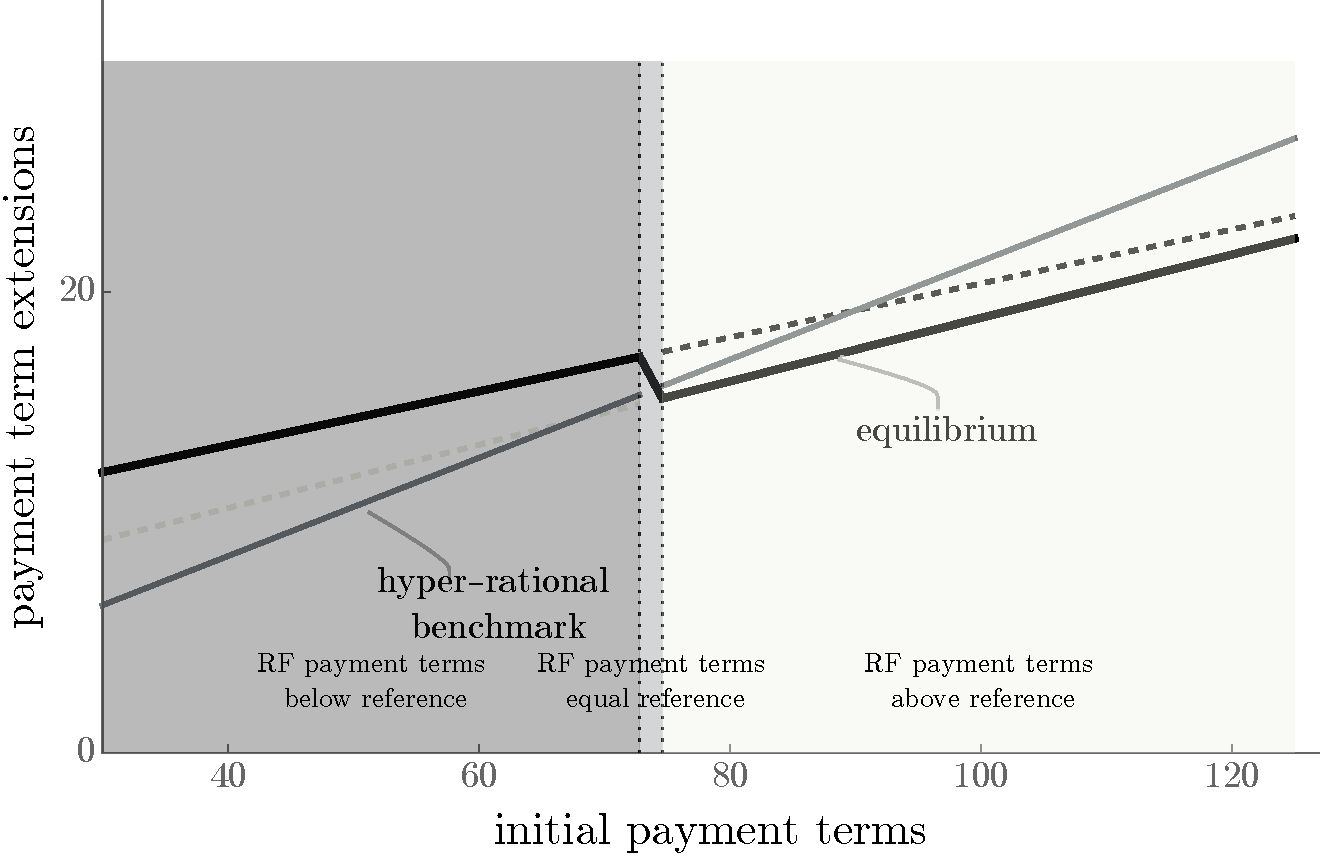
\includegraphics[width=\textwidth]{figures/06_ExtensionFairness_2.pdf}
         \caption{Weak fairness motive\newline ($\beta>0, \gamma>0$) \vspace{12pt}}
         \label{fig:delta:rational:dominant}
     \end{subfigure}
     \newline
     \begin{subfigure}[b]{0.48\textwidth}
         \centering
         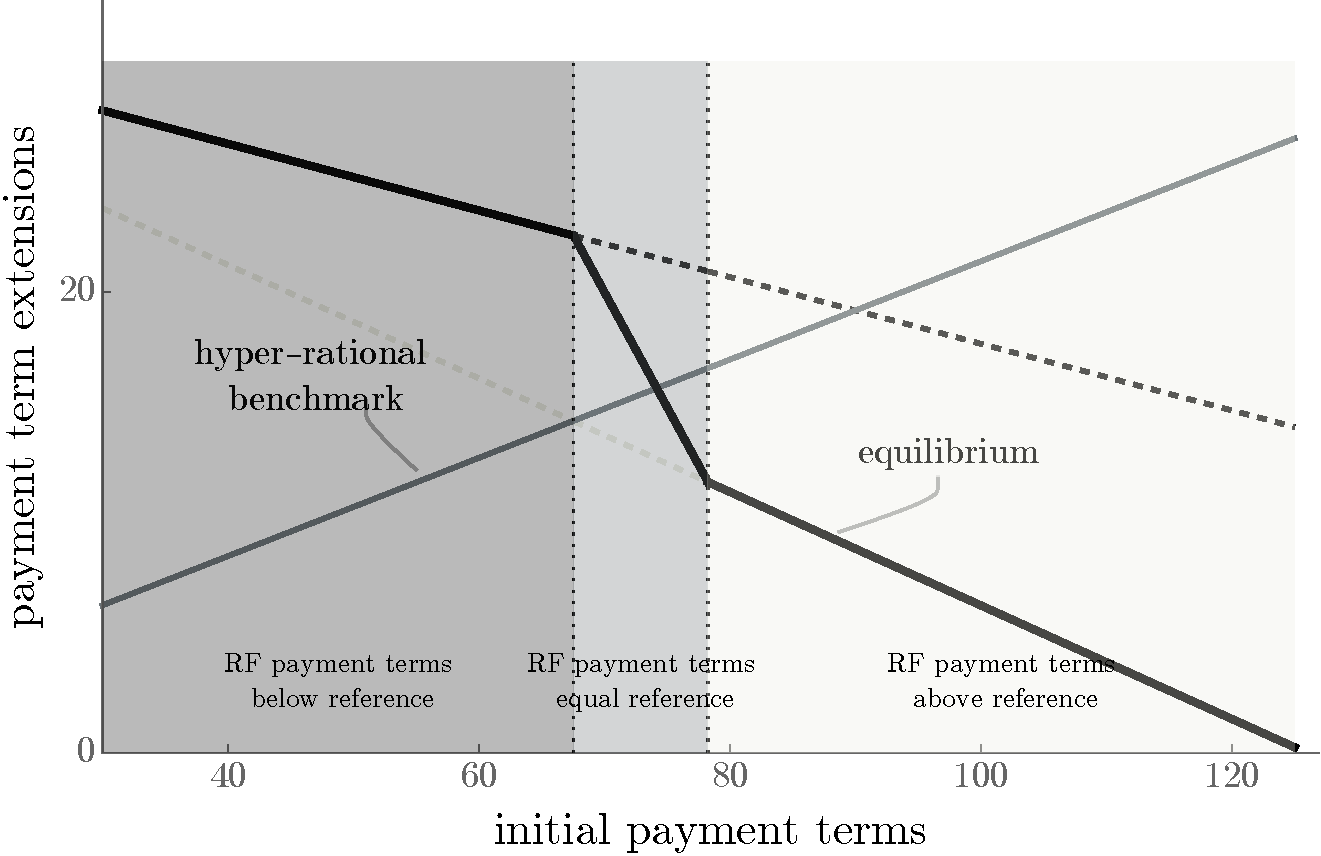
\includegraphics[width=\textwidth]{figures/06_ExtensionFairness_1.pdf}
         \caption{Strong fairness motive\newline ($\beta>0, \gamma>0$) \vspace{12pt}}
         \label{fig:delta:fair}
     \end{subfigure}
     \hfill
     \begin{subfigure}[b]{0.48\textwidth}
         \centering
         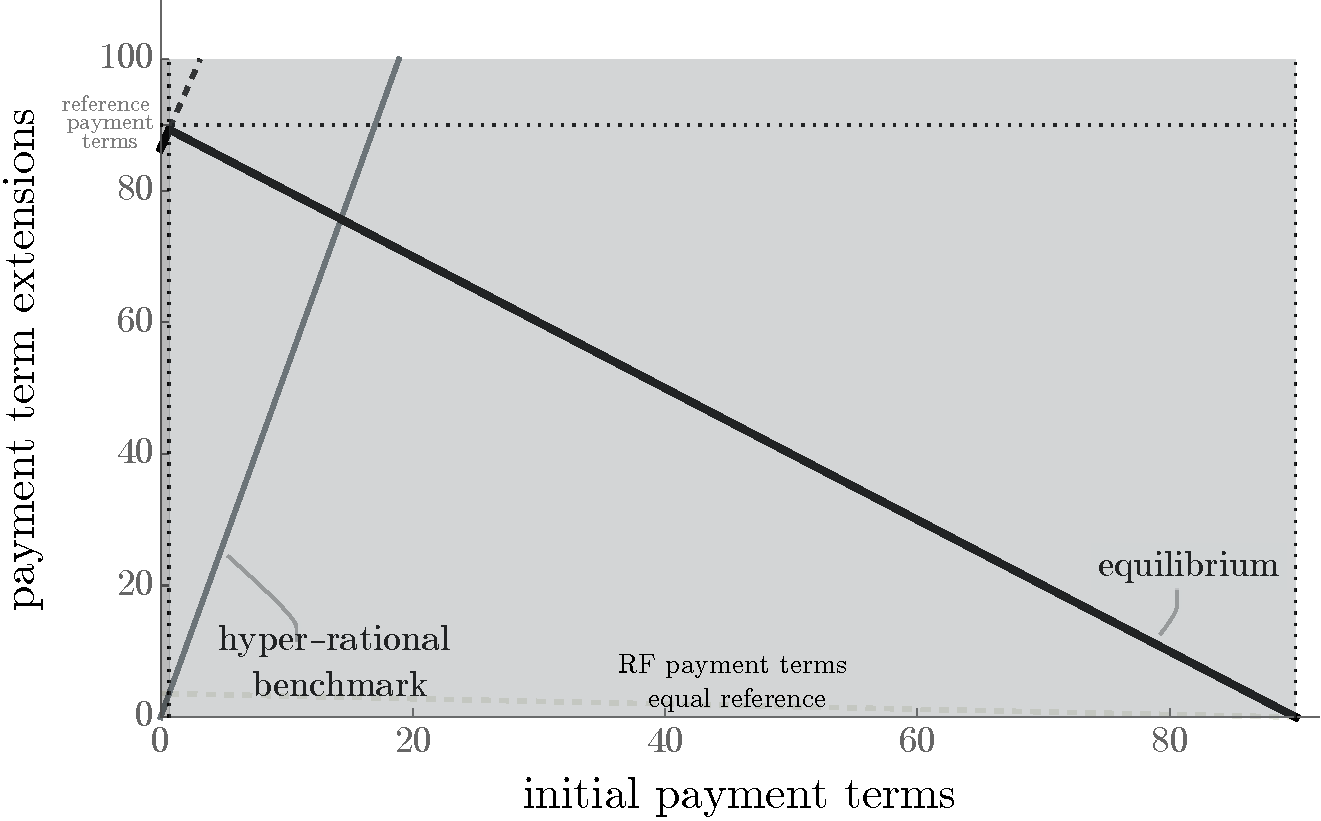
\includegraphics[width=\textwidth]{figures/06_ExtensionFairness_3.pdf}
         \caption{dominant fairness motive \newline($\beta\rightarrow\infty,\gamma\rightarrow\infty$)\vspace{12pt}}
         \label{fig:delta:fair:full}
     \end{subfigure}
        \caption{Varying fairness motive levels: payment term extensions for $\lambda=0$.}
        \label{fig:delta}
\end{figure}
This figure is suggestive of three ideas: (i) payment term extensions are always positive, (ii) longer initial payment terms can lead to longer or shorter extensions, (iii) the stronger the fairness motive, the larger the negative impact of initial payment terms. To capture these observations, we provide three formal results grounded in Proposition~\ref{prop:fairness}, respectively.
\begin{corollary}\label{cor:pos.extensions}\singlespacing
If $\lambda=0$ then $d^{f}_r - d_0 \geq 0$.%
\end{corollary}
\newpage
\begin{corollary}\label{cor:ptx.d0}\singlespacing
     Suppose $\beta>0$,  $\gamma>0$ and $\lambda=0$.%     
    \begin{enumerate}[label=(\roman*)]
        \item Unless $i_s \in\left\{\frac{i_b \alpha + \beta}{i_b\alpha + \beta\alpha}i_r,i_r + \gamma\right\}$, $\frac{\partial }{\partial d_0}\left(d^f_h\left(d_0\right)-d_0\right)>0$ if
            \begin{enumerate}[label=(\alph*)]
                \item $d_0 < \frac{ i_r (i_b + \alpha \beta)}{  i_b (i_r + \left(i_s- i_r\right) \alpha) + i_s \alpha \beta)}\dref$ and $i_s   >\frac{i_b \alpha + \beta}{i_b\alpha + \beta\alpha}i_r$ , or 
                \item $d_0 >\frac{ i_r + \left(1- \alpha\right) \gamma}{i_r + (i_s-i_r) \alpha + (1-\alpha)\gamma}\dref$ and $ i_s>i_r + \gamma$,
            \end{enumerate}
            and $\frac{\partial }{\partial d_0}\left(d^f_h\left(d_0\right)-d_0\right)<0$  otherwise.
        \item Further,
            \begin{enumerate}[label=(\alph*)]
                 \item for sufficiently small $\gamma$ and $\beta$ payment terms extension increase in initial payment terms;
                 \item for sufficiently large $\gamma$ and $\beta$ and for $i_s\alpha<i_r$, payment term extensions decrease in initial payment terms. 
        \end{enumerate}
    \end{enumerate}     
\end{corollary}%
$\;$\vspace{-60pt}\\
\begin{corollary}\label{cor:relative.fairness}\singlespacing
    (a) For $d_0 < \frac{ i_r (i_b + \alpha \beta)}{  i_b (i_r + \left(i_s- i_r\right) \alpha) + i_s \alpha \beta)}\dref$, the larger $\beta$, the more negative the effect of initial payment terms on payment term extensions. (b) For $d_0 > \frac{ i_r + \left(1- \alpha\right) \gamma}{i_r + (i_s-i_r) \alpha + (1-\alpha)\gamma}\dref$, the larger~$\gamma$, the more negative the effect of initial payment terms on payment term extensions.
\end{corollary}%
%
%


\subsection{Standardization motive}
Finally, we present the full model analysis by allowing $\lambda>0$.
\begin{proposition}[Full model]\label{prop:full}\singlespacing
    Suppose $\beta>0$, $\gamma>0$, and $\lambda>0$. There exists $\lambda_0$, $\underline{d}\left(\lambda_0\right)$ and $\overline{d}\left(\lambda_0\right)$ such that $\underline{d}\left(\lambda_0\right)<\frac{ i_r (i_b + \alpha \beta)}{
  i_b (i_r + \left(i_s- i_r\right) \alpha) + i_s \alpha \beta)}\dref$ and $\overline{d}\left(\lambda_0\right)>\frac{ i_r + \left(1- \alpha\right) \gamma}{i_r + (i_s-i_r) \alpha + (1-\alpha)\gamma}\dref$ and such that
    \begin{equation}
        d^{*}_r: = \begin{cases}
        \dHyp + \frac{(\dref-d_0) (1 - \alpha) \beta}{i_b + \beta}
  & \text{, if } d_0 < \underline{d}\left(\lambda_0\right)\\
  \dref & \text{, if }d_0\in\left[\underline{d}\left(\lambda_0\right),\overline{d}\left(\lambda_0\right)\right]\\
  \dHyp-\frac{(d_0 i_s-\dref i_r) \alpha \gamma}{i_r (i_r + \gamma)} & \text{, if } d_0 >\overline{d}\left(\lambda_0\right)
        \end{cases}
    \end{equation}
    is the unique bargaining outcome.
\end{proposition}
Structurally, this result resembles Proposition~\ref{prop:fairness}. It can be shown that even for $\beta=\gamma=0$, a range of initial payment terms exists such that for all $d_0$ in this range, both parties agree on the reference point. However, the standardization motive leads to a different impact of initial payment terms on extensions outside the range of perfect standardization. Figure~\ref{fig:standardization} illustrates this. %
\begin{figure}[ht]
     \centering
     \begin{subfigure}[b]{0.47\textwidth}
         \centering
         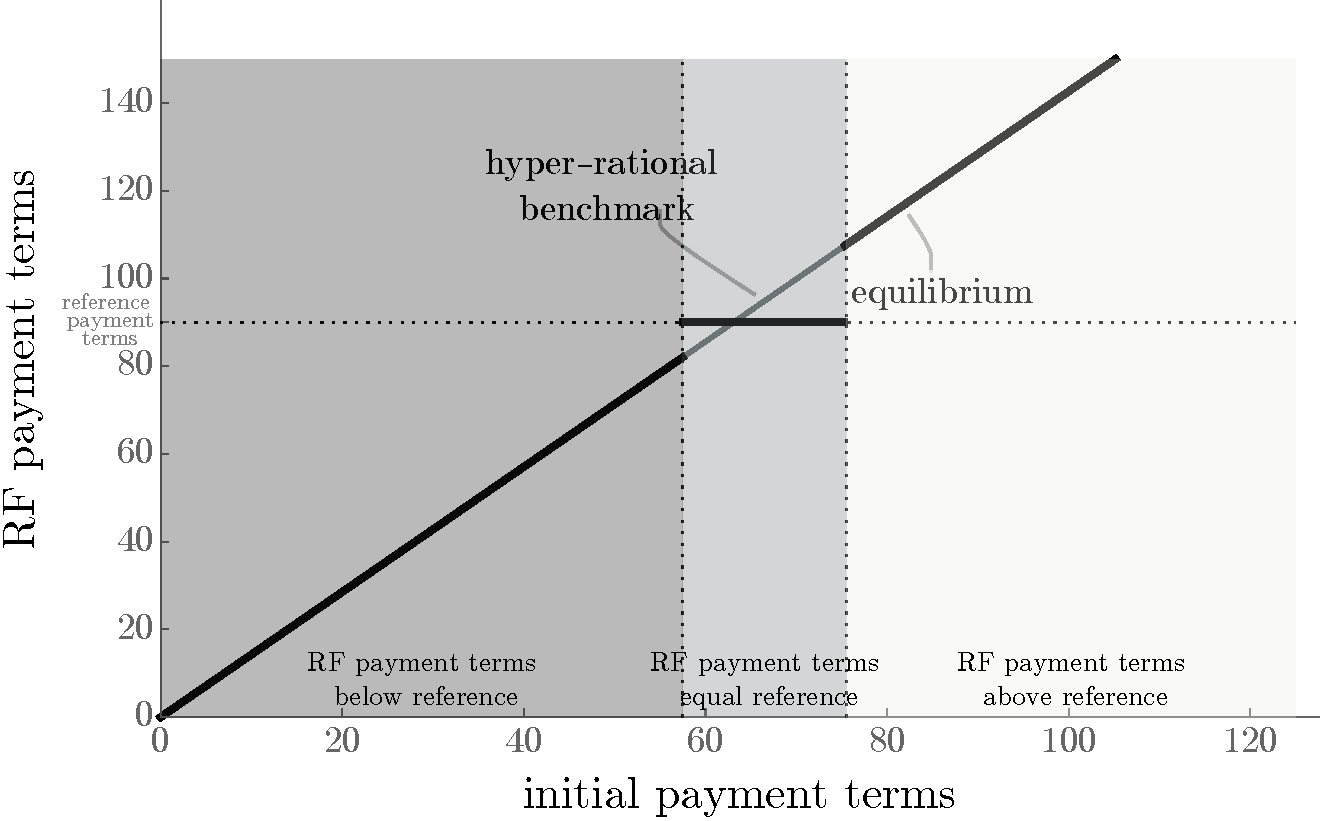
\includegraphics[width=\textwidth]{figures/10_PosteriorTermsStandard.pdf}
         \caption{RF payment terms \vspace{12pt}}
         \label{fig:standardization:dr}
     \end{subfigure}%
     \hfill%
     \begin{subfigure}[b]{0.47\textwidth}
         \centering
         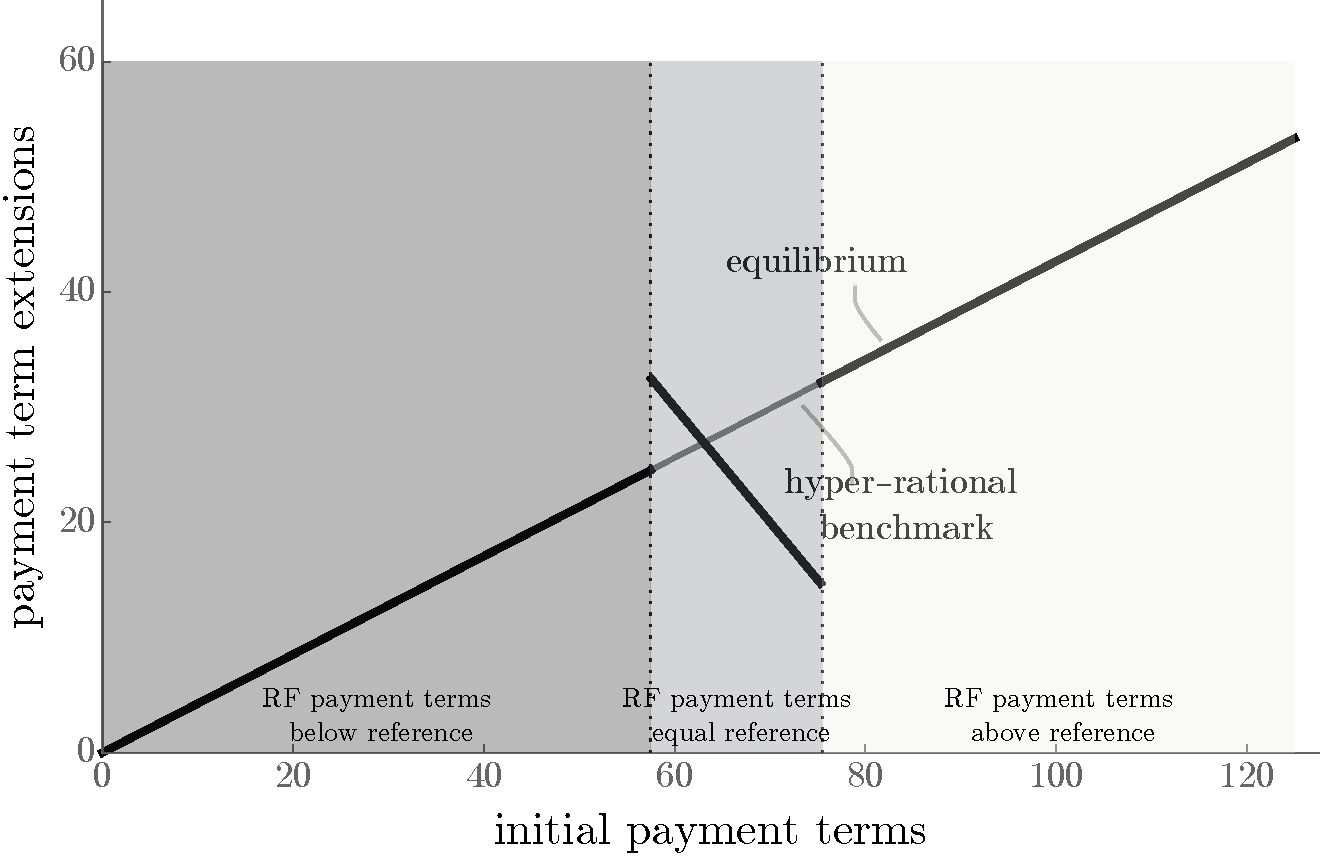
\includegraphics[width=\textwidth]{figures/10_ExtensionStandard.pdf}
         \caption{payment term extensions\vspace{12pt}}
         \label{fig:standardization:ext}
     \end{subfigure}
        \caption{Standardization motive, $\lambda>0, \gamma=\beta=0$.}
        \label{fig:standardization}
\end{figure}
To isolate the impact of the standardization motive, in this figure, we omit the fairness motive ($\beta=\gamma=0$). Unless the reference point is close enough to the hyper-rational bargaining outcome, both parties agree on the latter. Turning to the impact on payment term extensions,

\begin{corollary}\singlespacing\label{cor:standardization}
    Let $\lambda_0,\underline{d}\left(\lambda_0\right),$ and $\overline{d}\left(\lambda_0\right)$,  be defined as in Proposition~\ref{prop:full}.
    \begin{enumerate}[label=(\roman*)]
         \item For $d_0\in\left[\underline{d}\left(\lambda_0\right),\frac{ i_r (i_b + \alpha \beta)}{
  i_b (i_r + \left(i_s- i_r\right) \alpha) + i_s \alpha \beta)}\dref\right]$, standardization benefits, $\lambda$ lead to longer RF payment term extensions.
         \item For $d_0\in\left[\frac{ i_r + \left(1- \alpha\right) \gamma}{i_r + (i_s-i_r) \alpha + (1-\alpha)\gamma}\dref,\overline{d}\left(\lambda_0\right)\right]$, standardization benefits, $\lambda$ lead to shorter RF payment term extensions.
     \end{enumerate}
\end{corollary}

Standardization benefits, thus, do not necessarily imply that buyers are willing to forego benefits. The theoretical prediction is that there are cases in the cooperative bargaining approach where the supplier considers the buyer's benefits, leading to longer extensions to obtain standardized terms. Still, if the buyer has sufficient power, the standardization motive tends to favor shorter payment term extensions, as seen in the final result.
\begin{corollary}\label{cor:alpha:limit}
    Let $\beta=\gamma=0$. For $ \alpha\rightarrow 1$, standardization benefits, $\lambda$, always lead to (weakly) shorter RF payment terms.
\end{corollary}

\renewcommand\thehypothesis{\arabic{pretheorem}}
\section{Hypotheses}
The analytical results in Section~\ref{sec:model} allow for various predictions that we seek to test empirically. In line with all analytical models that we are aware of \citep[e.g.,][]{Serrano2018,vanderVliet2015,Tanrisever2012,Wuttke2016}, Corollary~\ref{cor:pos.extensions} predicts a positive extension of payment terms also in our model. To test this empirically, we hypothesize,
\theoremgroup
\begin{hypothesis}\label{H:expand}\singlespacing
The adoption of RF is associated with an extension of payment terms.
\end{hypothesis}
The subsequent discussion depends on the strength of the three motives. We argue that ex-ante, it is unclear which one will dominate, leading to two competing hypotheses. If the financing cost motive dominates the sample, then Corollary~\ref{cor:ptx.d0} suggests that payment term extensions increase in initial payment terms (see Figure~\ref{fig:delta:rational:full}). This follows the logic inherent to extant models where longer initial payment terms imply larger supplier benefits and, thus, a larger willingness to adopt RF even with long payment term extensions \citep{Grueter2017,vanderVliet2015,Tanrisever2012,Wuttke2016}. 
\theoremgroup
\renewcommand\thehypothesis{\arabic{pretheorem}\alph{hypothesis}}
\begin{hypothesis}\label{H:d0.pos}\singlespacing
Longer initial payment terms are associated with \underline{longer} extensions of payment terms under RF. 
\end{hypothesis}

Although the financing cost motive is present in virtually all RF programs, it can be weaker than what one might expect intuitively. Our sample features data from 2010 until 2019, and interest rates were historically low then. Typically, annual RF interest rates were about 2\%, corresponding to 2\%/365 $\approx$ 0.005479\%  daily interest rates. Suppose a buyer has an annual spend to a supplier of \$1,000,000. Then, this interest rate corresponds to about \$55 per day. This amount is arguably insufficient to cause major disputes in negotiations. No buyer or supplier would seriously threaten to end negotiations due to \$55 when facing revenues of \$1,000,000. So, a day more or less does not matter (of course, eventually, there is a limit to this argument, and suppliers will not agree to excessive extensions). When the financing cost motive is less salient, which likely applies to the sample period, we expect the fairness and standardization motives to be relatively stronger. Managers might even be inclined to ignore the financing costs and propose the same fair and standard terms for all suppliers. Following Corollaries~\ref{cor:ptx.d0} and~\ref{cor:standardization}, we thus propose the alternative hypothesis,
\begin{hypothesis}\label{H:d0.neg}\singlespacing
Longer initial payment terms are associated with \underline{shorter} extensions of payment terms under RF. 
\end{hypothesis}
To examine the mechanism further, we examine how different modes of RF impact the outcome. Suppliers can decide between two modes: automatic or manual. Automatic refers to suppliers using RF for each invoice when the buyer approves it. Manual means that suppliers are informed whenever a buyer approves an invoice and then decide whether and when to use RF to convert the receivables into liquidity. By postponing this conversion, suppliers reduce the financing costs linearly. Whereas the automatic approach is simpler, the manual one is more sophisticated, providing more flexibility to suppliers \citep{Grueter2017}. If suppliers strongly need liquidity, they likely opt for the automatic approach, the typical RF use case. This strong need for liquidity implies a weaker outside option. Consistent with our bargaining framework, we expect them to agree even to longer extensions than suppliers using RF manually. Formally,%
\theoremgroup%
\begin{hypothesis}\label{H:mode:direct}\singlespacing
Buyers bargain for longer payment terms with suppliers that use RF automatically than with those that use it manually.
\end{hypothesis}
Suppliers that choose a manual approach tend to focus more on financing aspects. After all, they follow a more sophisticated cash management strategy. In terms of Corollary~\ref{cor:ptx.d0}, this suggests relatively low $\gamma$ and, therefore, an overall more positive impact of initial payment terms on payment term extensions. Formally,
\begin{hypothesis}\label{H:mode:interact}\singlespacing
For suppliers that use RF manually, the impact of prior payment terms on extensions is more positive.
\end{hypothesis}
Turning to the standardization motive, Corollary~\ref{cor:standardization} predicts both a potentially positive and negative impact of standardization on payment term extensions. There are, however, some aspects that might favor a negative effect more. Standardization benefits arise for the buyer, not the supplier. So, one might expect the buyer rather than the supplier to concede to achieve standardization. Corollary~\ref{cor:alpha:limit} finds this analytically for powerful buyers. The analysis is less tractable if the buyer has less power.  Whereas Figure~\ref{fig:standardization} is only an illustration where the range of reductions due to standardization is longer than the range for extension, varying the parameters systematically, we find a consistent pattern. Considering the economic rationale, the fact that some buyers are quite powerful, and the numerical observation, we hypothesize,
\theoremgroup
\renewcommand\thehypothesis{\arabic{pretheorem}}
\begin{hypothesis}\label{H:standardization}\singlespacing
Payment terms get less extended when they become standardized.
\end{hypothesis}
Central to our model is the assumption that Nash bargaining takes place. The parameter $\alpha$ captures the buyer's bargaining power, which we expect to be affected by buyer experience. Whereas suppliers only adopt RF once with each buyer, each buyer can learn from past payment term negotiations and accumulate more bargaining power. Since bargaining power is, in general, associated with a more favorable outcome for the buyer, we expect,
\theoremgroup
\begin{hypothesis}\label{H:experience}\singlespacing
Buyer experience has a positive impact on payment term extensions.
\end{hypothesis}
Finally, let us take a more aggregate view. If the fairness and standardization motives apply, we would expect harmonization. Even if suppliers differ in their initial payment terms, those differences might vanish. If the data is consistent with our model, we expect,
\theoremgroup
\renewcommand\thehypothesis{\arabic{pretheorem}\alph{hypothesis}}
\begin{hypothesis}\label{H:reduceTerms}\singlespacing
The adoption of RF is associated with a reduction rather than an increase in different levels of payment terms.
\end{hypothesis}
Relatedly, we expect the harmonization to be heterogenous across all buyers. Standard terms are less salient in smaller programs, and forming a consistent reference point is more difficult. Buyers with larger programs might also have a stronger incentive to standardize terms. Therefore, we expect program size to affect buyers' likelihood of reducing the number of different payment terms, that is, to standardize. Formally,
\begin{hypothesis}\label{H:salience}\singlespacing
Buyers with larger RF programs are more likely to standardize payment terms.
\end{hypothesis}





\section{Data}\label{sec:data}
Our primary data source is a leading, U.S.-based RF provider, which runs RF programs with large global buyers. Each program contains multiple suppliers, but each supplier is only in one program in this dataset. The RF provider does not charge any setup, operating, or consulting fees, but the RF interest rate includes a fee. RF programs have a long-term focus. So far, no active supplier in this sample has left the program, and the earliest dyad has existed for about ten years. Once a supplier joins a program, the program handles all transactions.

RF requires buyers to disclose a series of essential variables, such as buyer industry and buyer revenue. About 75\% of the suppliers are private firms with no publicly available data; for RF, they do not need to inform the RF provider with the same level of details. Nevertheless, some supplier-level variables are still available in this dataset because each RF program features an RF platform. Buying firms can enter variables such as the initial payment terms and RF payment terms, as well as supplier industry, country, and revenue. The initial payment terms refer to the latest payment terms before adopting RF; the RF payment terms refer to the payment terms that both parties agreed on when introducing RF. Buyers do not record the supplier's interest rate outside RF, however. As we learned from the RF provider, suppliers are unwilling to disclose this information due to their concern that buyers or providers might use this sensitive information to their disadvantage in the long run. Few suppliers have a publicly documented credit rating, so the RF provider does not collect this variable.

The data refer to a period from 2010 to 2019, with 73 buyers and 1,898 buyer-supplier dyads with complete data. As the data collection ended in December 2019, none of the effects in our study were affected by the COVID-19 pandemic. We used an earlier version of this dataset to investigate a different research question with other hypotheses and a different dependent variable \citep{Wuttke2019}. In that former study, we investigated the speed at which suppliers adopt RF. In that study, independent variables explain the time between being offered RF and using it. In contrast, in this present study, payment term extension is the dependent variable. In addition, the former research draws from theory on technology adoption, whereas this present study tests analytical predictions. For consistency, we followed the exclusion criteria of \citet{Wuttke2019} and removed extreme outliers (three interquartile ranges below (above) the first (third) quartile). The data still differs slightly since we use a more recent dataset. As one robustness check and for consistency, we examine our main model using the exact same dataset as in \citet{Wuttke2019}.

We complemented this dataset with publicly available data. We used the London Interbank Offered Rate (LIBOR), a widely accepted reference rate for the short-term interest rate, to measure the risk-free rate. We use LIBOR data from the Federal Reserve Bank (St. Louis). The RF provider shared anonymous data without firm names for confidentiality reasons, which prevented us from collecting any further firm-level data.

\subsection{Variables}\label{sec:variables}
Table~\ref{tab:demographics} provides an overview of the demographic variables. To obtain fairly balanced categories for \textit{supplier country} and \textit{supplier industry}, we decided to pool countries with less than ten suppliers into the category `other countries'; this category captures mostly small EU countries such as Belgium, Sweden, and Latvia. Table~\ref{tab:demographics} also displays \textit{buyer country} and \textit{buyer industry}. These buyer-level demographic variables do not affect our primary analysis, so creating more balanced groups is unnecessary. The factor variable \textit{year} captures when a supplier agrees to adopt RF.

Table~\ref{tab:variableSummary} provides summary statistics for the continuous variables. The variable \textit{payment term extensions} captures the difference between \textit{RF payment terms} and \textit{initial payment terms}. In a few cases, buyers adopt RF even with shorting payment terms (i.e., negative extensions), but the mean is positive with $55.6$ days. The value of \textit{initial payment terms} averages $52.6$ days, \textit{RF payment terms} averages $108.2$ days. \textit{RF interest rate} averages about 2\%. Suppliers that use RF incur this rate plus the \textit{risk-free rate}, which averages 1.1\%. These are annualized values. To operationalize standardization, we calculated for each buyer the most frequent RF payment term (e.g., 60 days). Each supplier with RF payment terms equal to this value is coded as receiving standard terms; precisely, the variable \textit{standard terms} assumes one and zero otherwise. Its mean of 58.5\% indicates that about one out of two suppliers obtained standard terms in our sample. \textit{Annual spend} captures sales within the buyer-supplier dyad, whereas \textit{supplier revenue} is a supplier's entire revenue so that it may also originate from other buyers. These two variables are right-skewed, so we consider their logarithm in the subsequent analysis. Buyers tend to be larger than suppliers in our dataset, as reflected by a higher average \textit{buyer revenue}. The variable \textit{buyer costs of goods sold} indicates the importance of the buyers' upstream supply chains.%
\begin{table}[ht]
{
\scalebox{1}{%
\begin{tabular}{%
lc@{\hspace{.2em}}rc@{\hspace{.2em}}rc@{\hspace{.9em}}lc@{\hspace{.2em}}rc@{\hspace{.2em}}rc
}\toprule\\[-12pt]
supplier country && {count} && {percentage} && supplier industry && {count} && {percentage} \\ \cline{1-5} \cline{7-11}\\[-12pt] 
 Canada && 25 && 1.32\% && Administrative support && 4 && 0.21\% \\[3pt] 
 Denmark && 39 && 2.05\% && Automobiles and parts && 11 && 0.58\% \\[3pt] 
 Germany && 905 && 47.68\% && Basic resources && 115 && 6.06\% \\[3pt] 
 Mexico && 134 && 7.06\% && Chemicals && 29 && 1.53\% \\[3pt] 
 Netherlands && 17 && 0.90\% && Construction and materials && 78 && 4.11\% \\[3pt] 
 Other && 59 && 3.11\% && Health care && 19 && 1.00\% \\[3pt] 
 Slovenia && 11 && 0.58\% && Industrial goods and services && 1188 && 62.59\% \\[3pt] 
 Switzerland && 24 && 1.26\% && Media && 106 && 5.58\% \\[3pt] 
 United Kingdom && 27 && 1.42\% && Not indicated && 141 && 7.43\% \\[3pt] 
 United States && 657 && 34.62\% && Oil and gas && 72 && 3.79\% \\[3pt] \cline{1-5}\\[-12pt] 
 \textbf{total} && 1898 && 100\% && Retail && 22 && 1.16\% \\[3pt] 
  &&  &&  && Technology && 113 && 5.95\% \\[3pt] \cline{7-11}\\[-12pt] 
 buyer country && {count} && {percentage} && \textbf{total} && 1898 && 100\% \\ \cline{1-5}\\[-12pt] 
 Australia && 1 && 1.37\% &&  &&  &&  \\[3pt] 
 Belgium && 1 && 1.37\% && buyer industry && {count} && {percentage} \\ \cline{7-11}\\[-12pt] 
 Canada && 3 && 4.11\% && Basic resources && 2 && 2.74\% \\[3pt] 
 Czech Republic && 4 && 5.48\% && Construction and materials && 17 && 23.29\% \\[3pt] 
 Denmark && 4 && 5.48\% && Consumer goods && 1 && 1.37\% \\[3pt] 
 Germany && 27 && 36.99\% && Health care && 10 && 13.70\% \\[3pt] 
 Ireland && 1 && 1.37\% && Industrial goods and services && 24 && 32.88\% \\[3pt] 
 Mexico && 5 && 6.85\% && Oil and gas && 15 && 20.55\% \\[3pt] 
 Sweden && 1 && 1.37\% && Public Administration && 1 && 1.37\% \\[3pt] 
 Switzerland && 6 && 8.22\% && Wholesale and retail && 3 && 4.11\% \\[3pt] \cline{7-11}\\[-12pt] 
 United Kingdom && 6 && 8.22\% && \textbf{total} && 73 && 100\% \\[3pt] 
 United States && 14 && 19.18\% &&  &&  &&  \\[3pt] \cline{1-5}\\[-12pt] 
 \textbf{total} && 73 && 100\% && year && {count} && {percentage} \\ \cline{7-11}\\[-12pt] 
  &&  &&  && 2010 && 136 && 7.17\% \\[3pt] 
 mode && {count} && {percentage} && 2011 && 129 && 6.80\% \\ \cline{1-5}\\[-12pt] 
 auto discount && 1608 && 84.72\% && 2012 && 137 && 7.22\% \\[3pt] 
 manual discount && 290 && 15.28\% && 2013 && 94 && 4.95\% \\[3pt] \cline{1-5}\\[-12pt] 
 \textbf{total} && 1898 && 100\% && 2014 && 127 && 6.69\% \\[3pt] 
  &&  &&  && 2015 && 167 && 8.80\% \\[3pt] 
  &&  &&  && 2016 && 349 && 18.39\% \\[3pt] 
  &&  &&  && 2017 && 256 && 13.49\% \\[3pt] 
  &&  &&  && 2018 && 186 && 9.80\% \\[3pt] 
  &&  &&  && 2019 && 317 && 16.70\% \\[3pt] \cline{7-11}\\[-12pt] 
  &&  &&  && \textbf{total} && 1898 && 100\% \\\bottomrule
\end{tabular}
}%scalebox
}
\caption{Summary statistics for categorical variables.}
\label{tab:demographics}
\end{table}%
\FloatBarrier
\begin{table}[thb]\vspace{16pt}
{
\scalebox{1}{%
\begin{tabular}{%
L{2.5in}c@{\hspace{.2em}}*{3}{R{0.55in}c@{\hspace{.2em}}}R{0.57in}c@{\hspace{.2em}}R{0.43in}c@{\hspace{.2em}}
}
\toprule
variable name  &&  min.  &&  max.  &&  mean  &&  std. dev.  &&  count\\[3pt]\midrule
payment term extensions (days) && -60.000 && 358.000 && 55.584 && 58.546 && 1898 \\[3pt]
 initial payment terms (days) && 0.000 && 180.000 && 52.599 && 28.107 && 1898 \\[3pt]
 RF payment terms (days) && 30.000 && 360.000 && 108.183 && 52.404 && 1898 \\[3pt]
 RF interest rate && 0.010 && 0.052 && 0.020 && 0.012 && 1898 \\[3pt]
 risk free rate && 0.002 && 0.028 && 0.011 && 0.009 && 1898 \\[3pt]
 standard terms (1=yes) && 0.000 && 1.000 && 0.585 && 0.493 && 1898 \\[3pt]
 annual spend (mn USD) && 0.000 && 212.874 && 1.825 && 5.794 && 1898 \\[3pt]
 supplier revenue (bn USD) && 0.000 && 15.405 && 0.082 && 0.735 && 1898 \\[3pt]
 buyer revenue (bn USD) && 1.000 && 75.000 && 12.130 && 15.553 && 73 \\[3pt]
 buyer costs of goods sold (bn USD) && 1.000 && 45.000 && 7.671 && 10.006 && 73 \\[3pt]
 RF program size (num. of suppliers) && 1.000 && 429.000 && 26.000 && 55.626 && 73 \\[3pt]
 buyer experience (count) && 0.000 && 428.000 && 71.189 && 100.405 && 1898 \\\bottomrule
\multicolumn{3}{L{0.5\textwidth}}{\footnotesize\textit{Note.  Values reported in this table are not transformed.}}
\end{tabular}
}%scalebox
}
\caption{Summary statistics for continuous variables.}
\label{tab:variableSummary}
\end{table}%
\FloatBarrier
The \textit{RF program size} variable reflects the number of suppliers in a buyer's program, with an average size of 26 suppliers (=1,898/73). Finally, the variable \textit{buyer experience (count)} indicates the number of suppliers that a buyer bargained with in the past. Although this variable is on the buyer level, there are 1,898 observations because it increases by 1 for each supplier. Because this count measure is right-skewed, we consider its logarithm.%,

We standardize all variables for the subsequent analysis (i.e., we mean-center each and divide it by its standard deviation)  with two exceptions. By keeping \textit{payment term extensions} and \textit{initial payment terms} unscaled (only mean-centered), we can attain a more meaningful interpretation.


\subsection{Econometric strategy}
We formulated the hypotheses such that they can be tested in reduced form since our dataset does not feature sufficient data for structural estimation. Such an approach would require data related to supplier-level variables, such as the supplier's fairness parameter ($\gamma$), and dyadic data, such as bargaining power ($\alpha$), which is not included in our dataset. Still, to illustrate our data and mimic the format of our theoretical predictions (Figures~\ref{fig:fair:dr} and~\ref{fig:delta}), we present the relationship between initial payment terms and payment term extensions for one buyer in Figure~\ref{fig:23:zones}. It is vital to see that the regions and solid lines are somewhat arbitrary in this figure, rather than a result of rigorous estimation. In contrast, the dashed lines result from an OLS estimation.

\begin{figure}[tb]
      \begin{subfigure}[b]{0.31\textwidth}
         \centering
         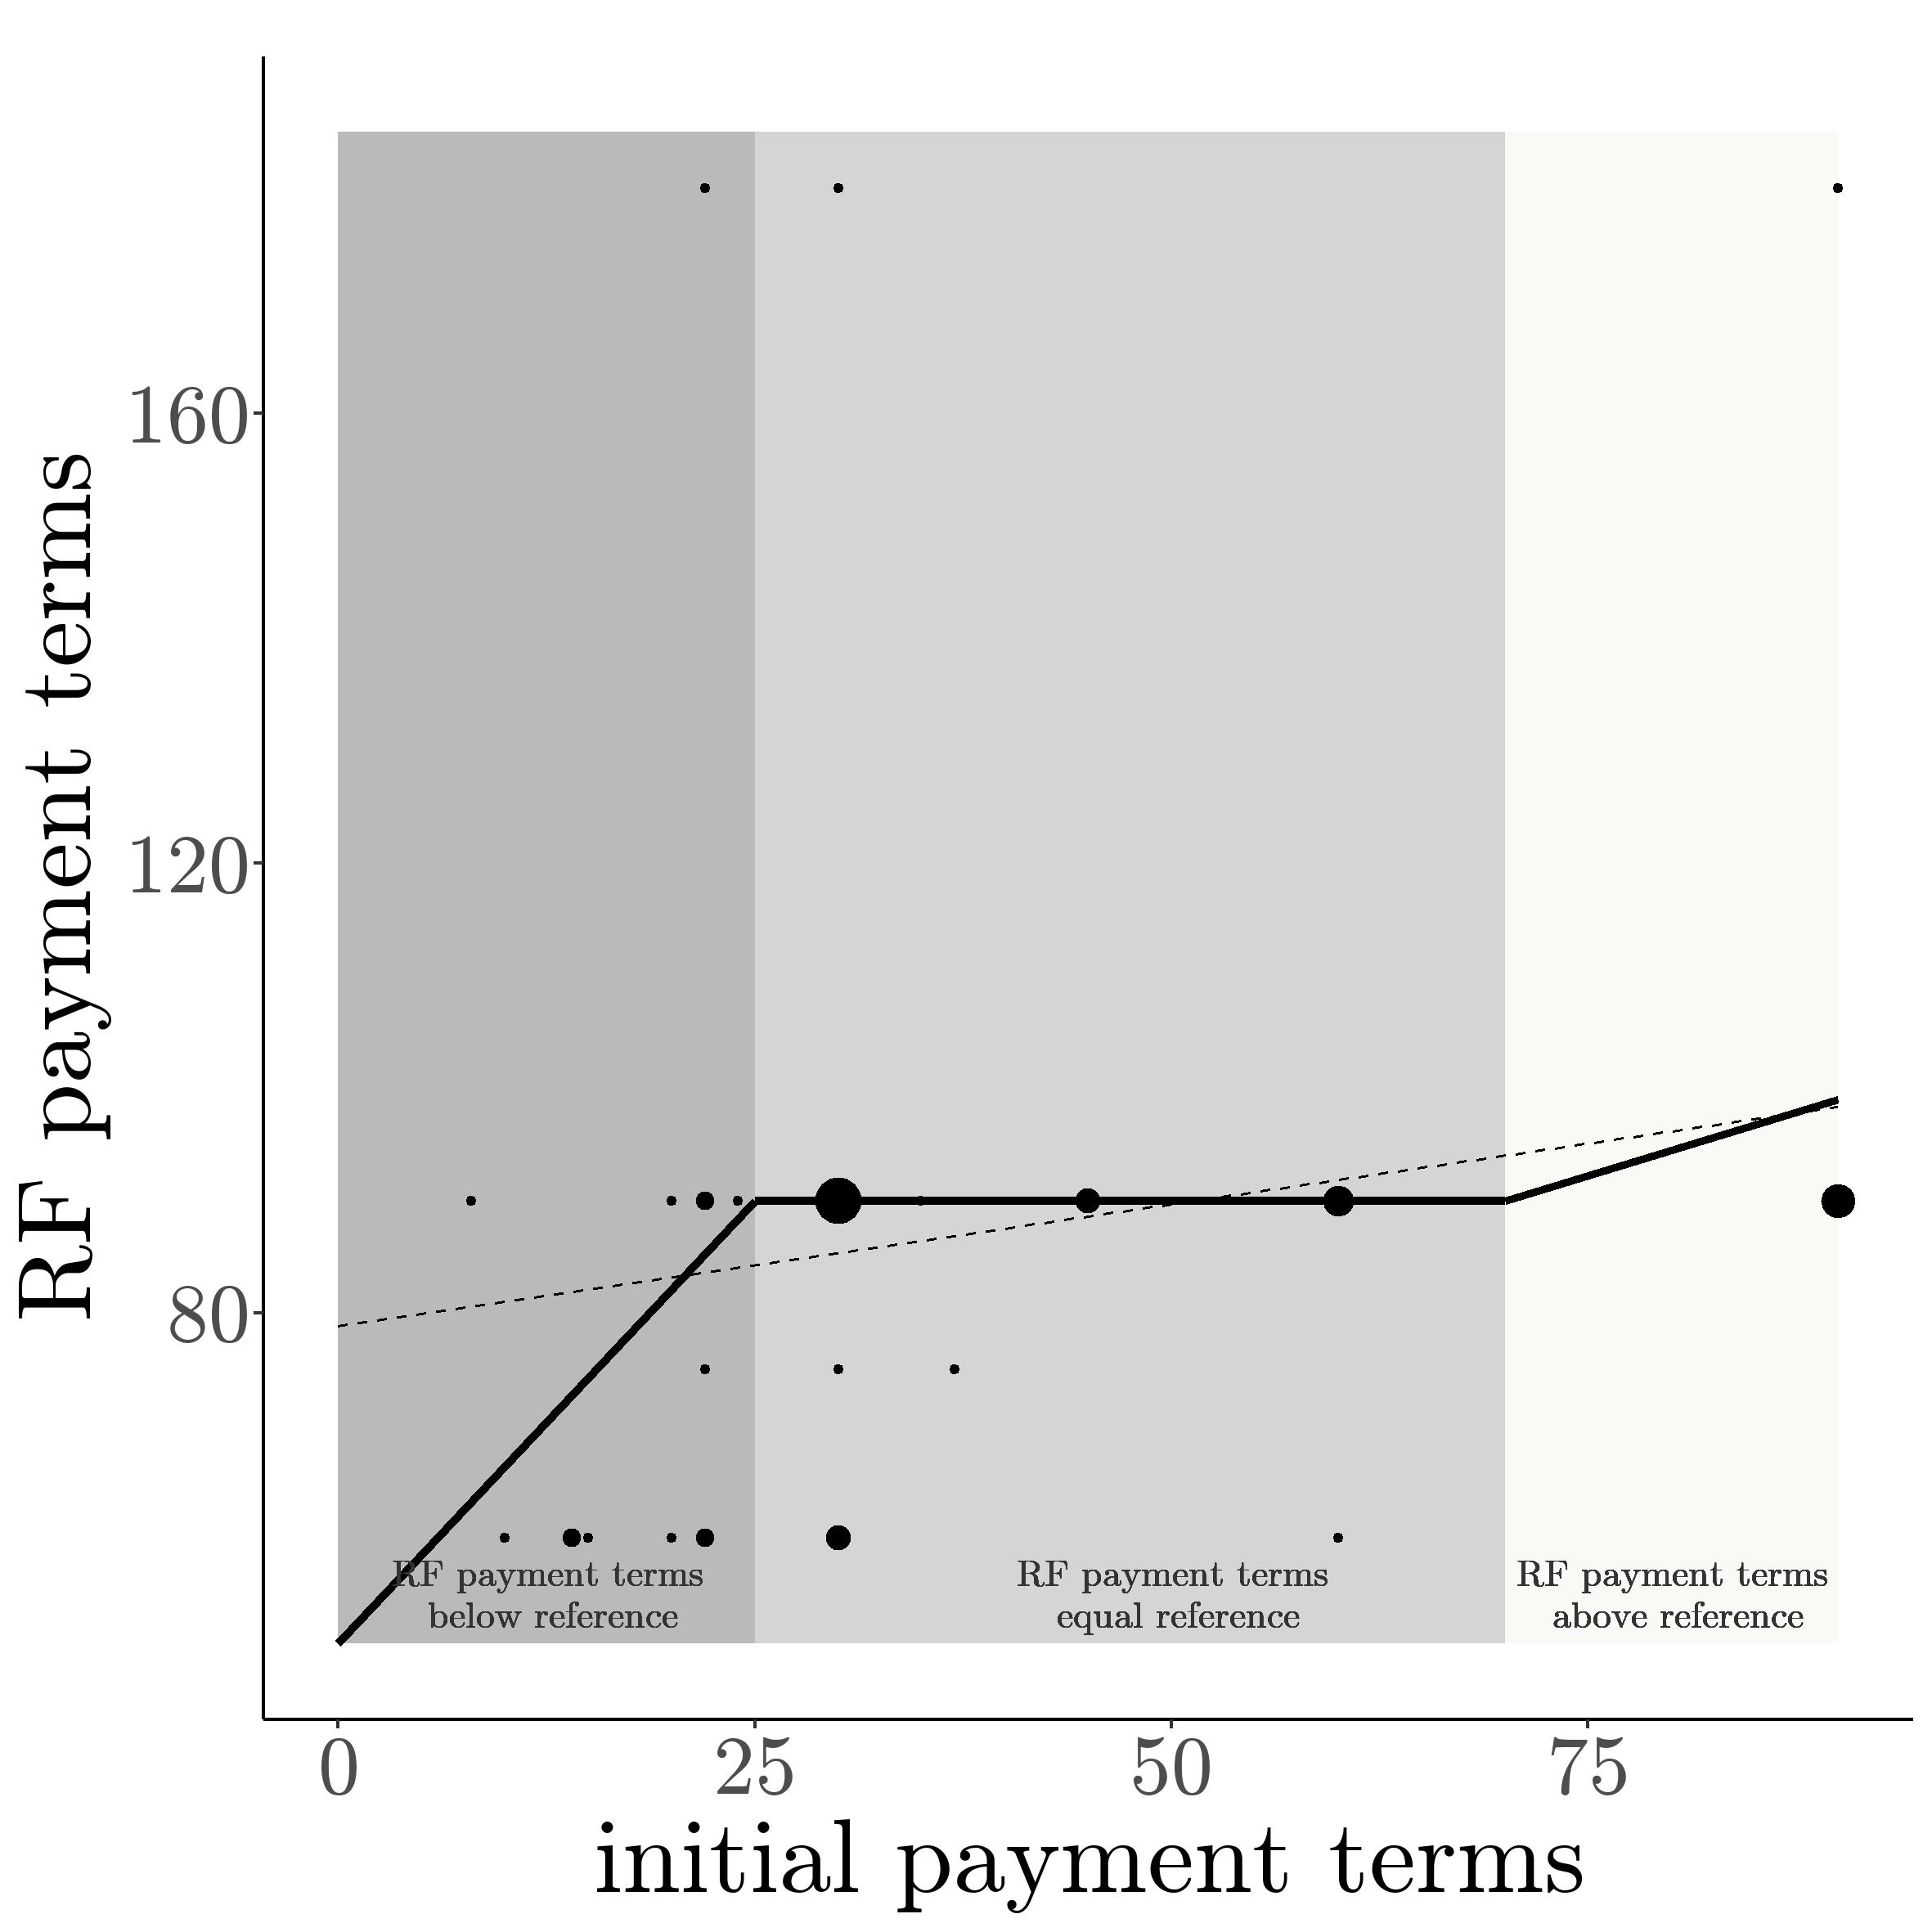
\includegraphics[width=\textwidth]{figures/bid_23_posterior.png}
         \caption{RF factoring payment terms. The solid line mimics the equilibrium curve in Figure~\ref{fig:fair:dr}. \vspace{18pt}}
         \label{fig:23:posterior}
     \end{subfigure}\hfill
     \begin{subfigure}[b]{0.31\textwidth}
         \centering
         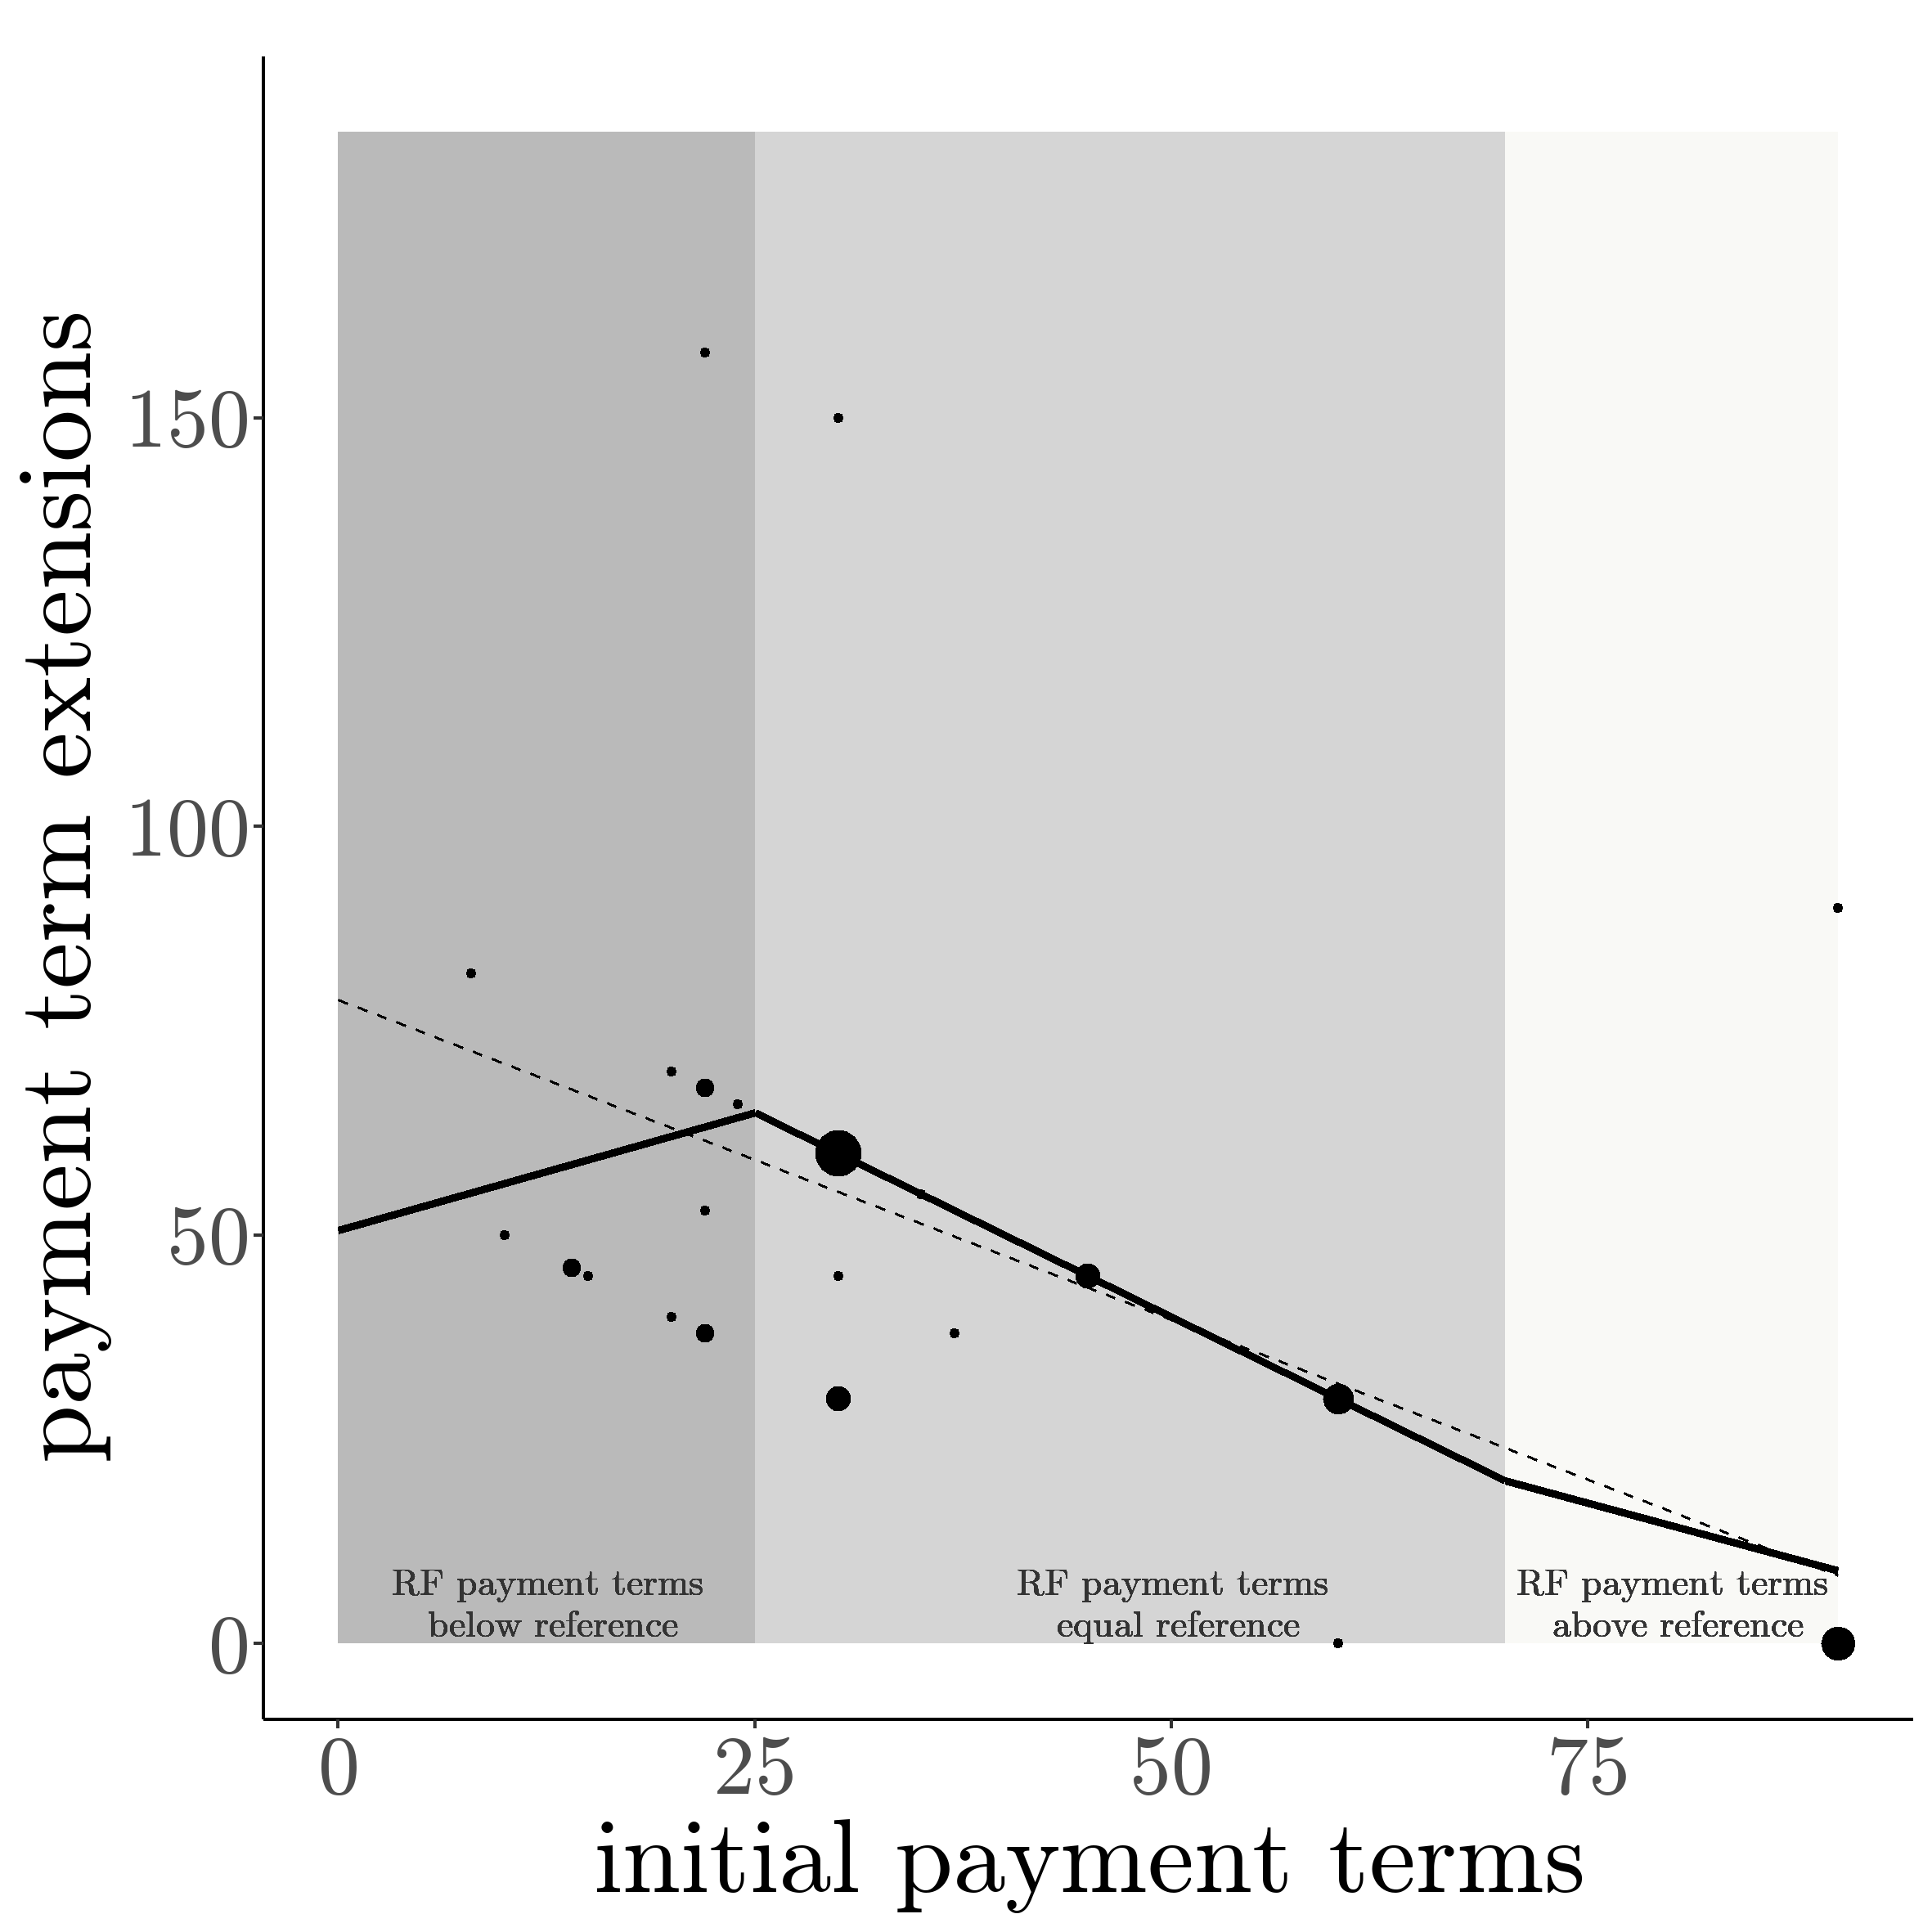
\includegraphics[width=\textwidth]{figures/bid_23_extension.png}
         \caption{Payment term extensions. The solid line mimics the equilibrium curve in Figure~\ref{fig:delta}. \vspace{18pt}}
         \label{fig:23:extension}
     \end{subfigure}\hfill
     \begin{subfigure}[b]{0.31\textwidth}
         \centering
         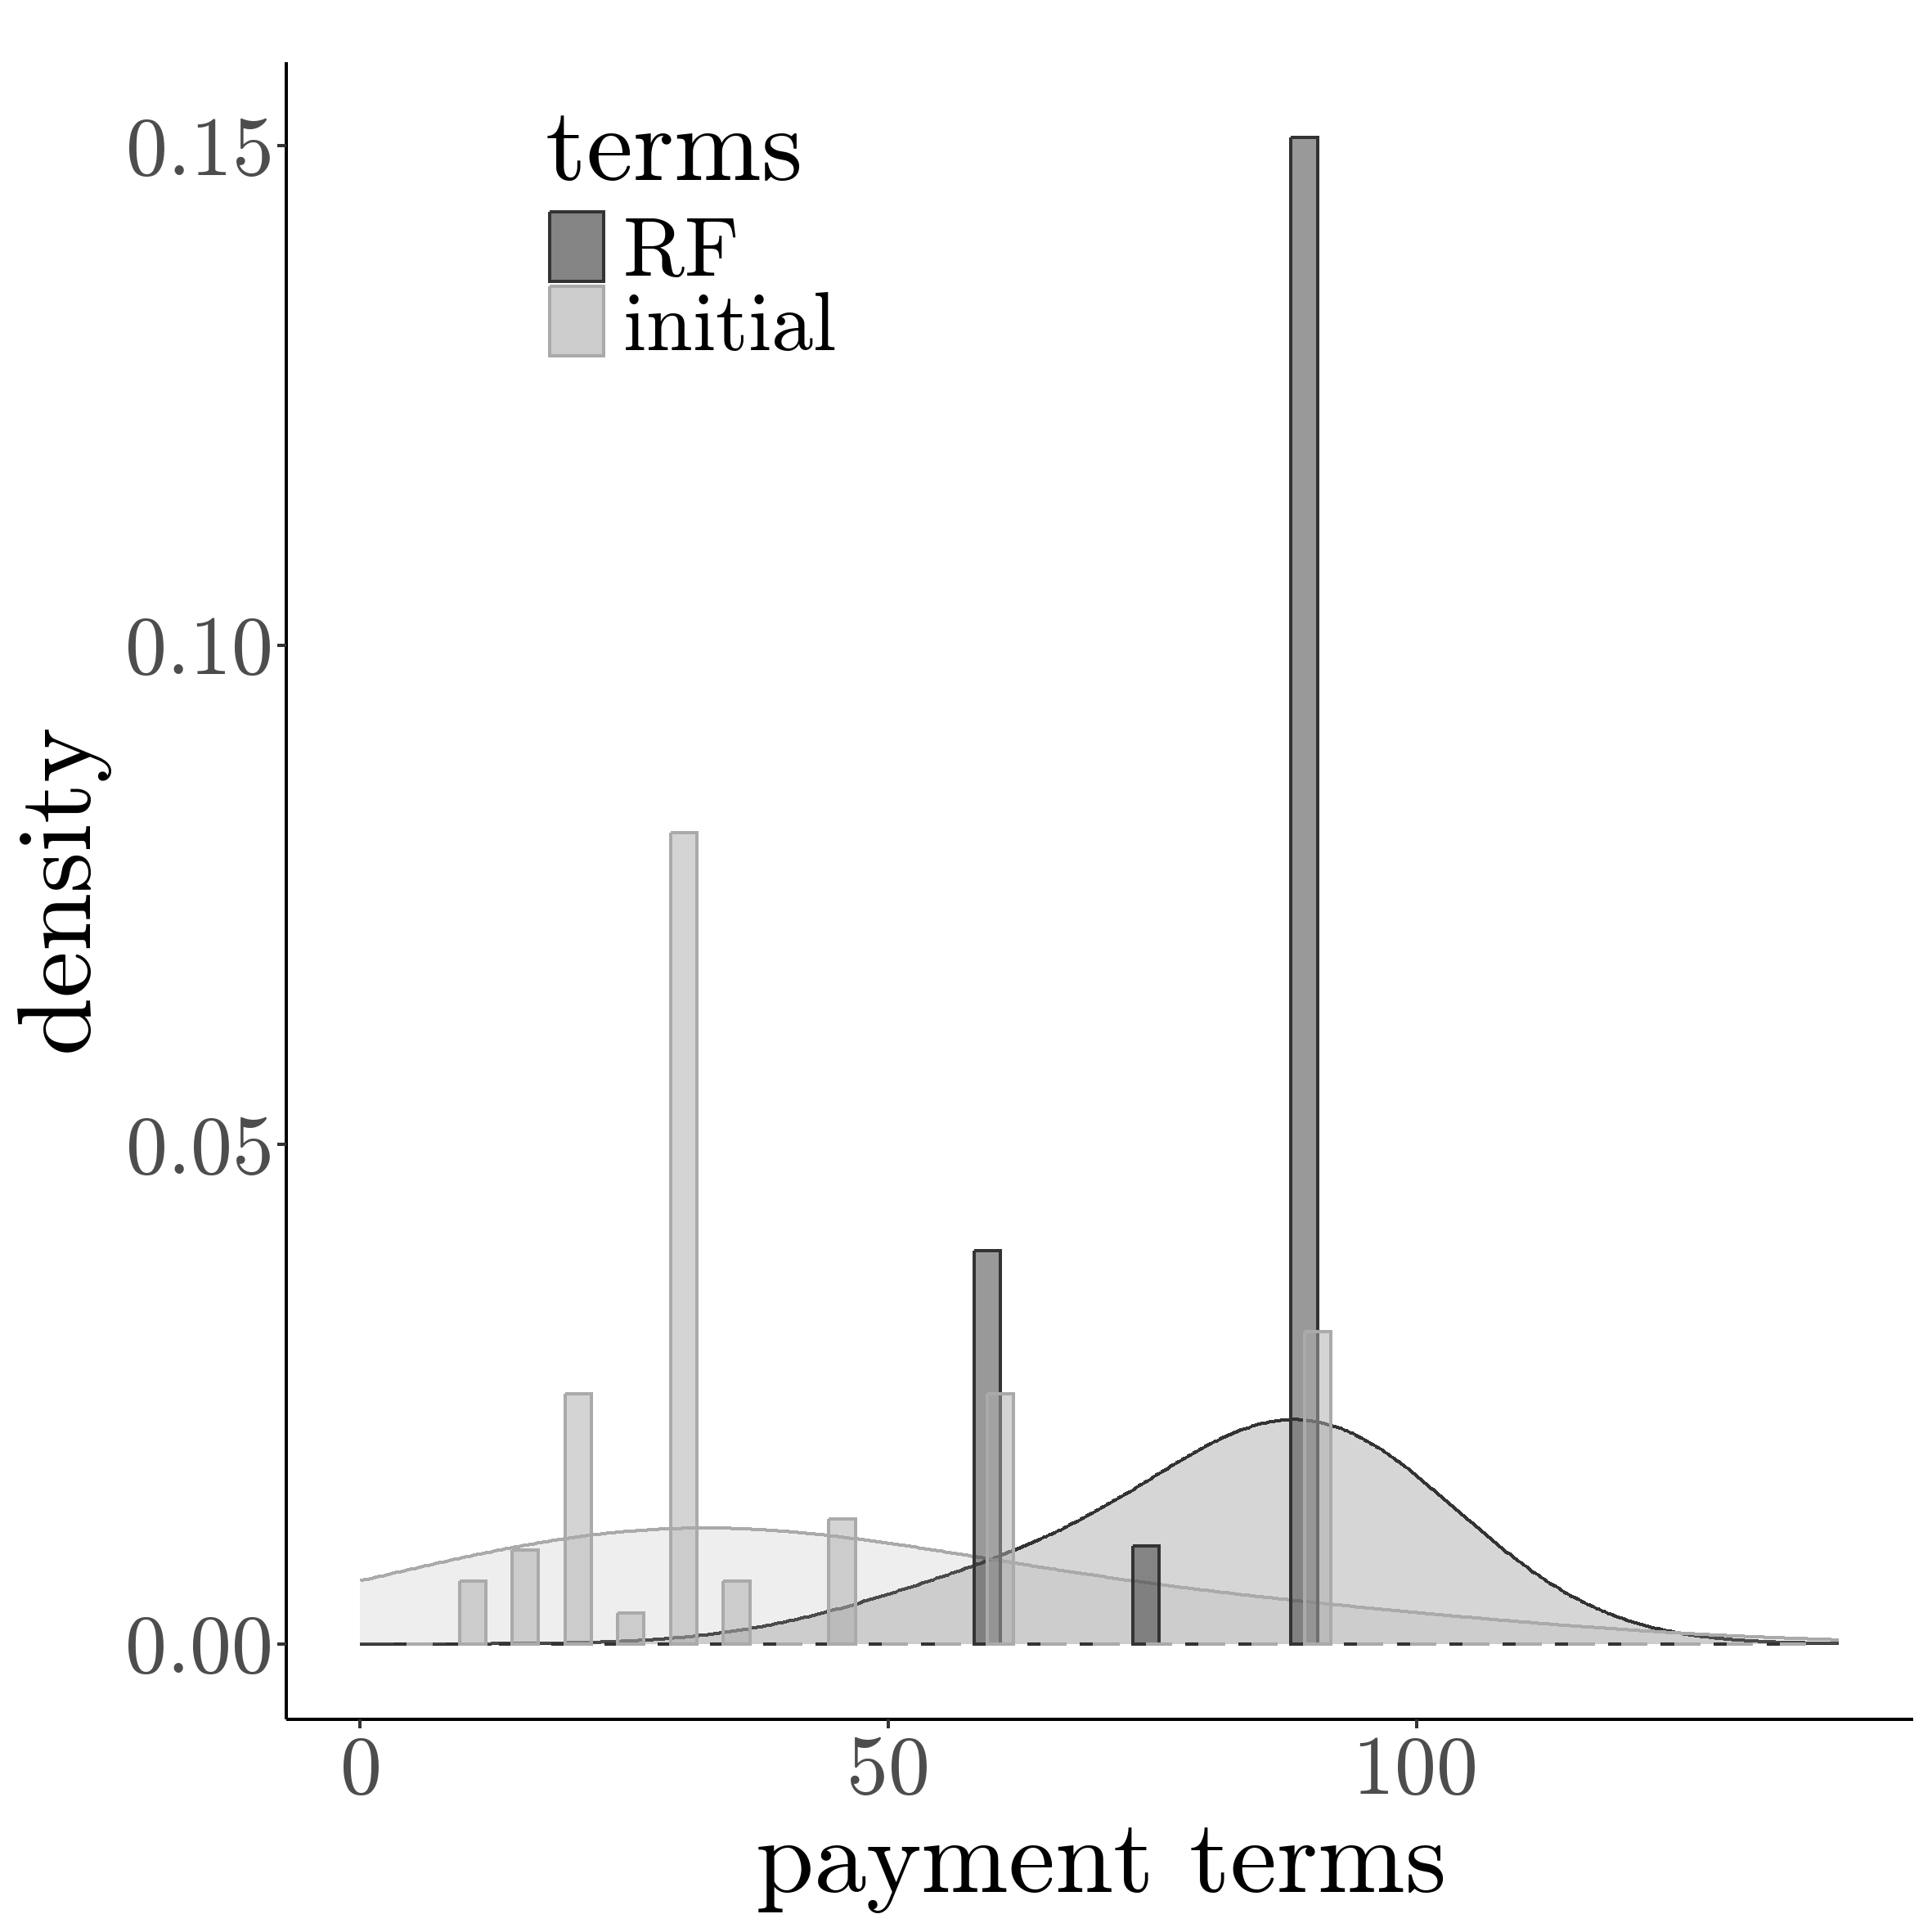
\includegraphics[width=0.95\textwidth]{figures/hist.pt.png}
         \caption{Histrogram and density of initial payment terms and RF payment terms.\vspace{18pt}}
         \label{fig:hist}
     \end{subfigure}
        \caption{Empirical example of one buyer with 64 suppliers in its RF program. Circle size indicates the number of suppliers. Dashed lines indicate OLS estimates for this buyer.}
        \label{fig:23:zones}        
\end{figure}
\newpage
Taking a slightly different perspective on the same buyer, Figure~\ref{fig:hist} presents the histograms of initial payment terms and RF payment terms along with normal density plots. For this buyer, it is suggestive of the idea that RF leads to longer payment terms and harmonization, reflected in fewer different terms and more frequent use of the new standard (here 90 days).
 
We test Hypothesis~\ref{H:expand} using a paired $t$-test and a non-parametric paired Wilcoxon-test. Hypotheses~2--5 are all on payment term extensions. To capture that each buyer offers RF to multiple suppliers in our sample, we test them consistently using a linear model with fixed effects on the buyer level (we also estimate a random effects model as a robustness test, see section~\ref{sec:robust}). The dataset spans almost a decade with potentially changing approaches. To capture this, we include \textit{year} as a factor variable in our model. Payment terms can differ by \textit{supplier country} and \textit{supplier industry}, so we include both variables on the supplier level. If the conditions are quite favorable (i.e., small \textit{RF interest rate}), one might expect long payment term extensions, so we include this variable. Our model also includes the \textit{risk free rate} to control the current financing situation. Since the fixed effects already capture all variables constant on the buyer level, the model does not contain any buyer-level time-invariant variables.  Because the \textit{annual spend} and \textit{supplier revenue} might also affect the bargaining outcome, we include both. We further include the variables required for testing Hypotheses~2--5, leading to,
\begin{dmath*}
    \text{Payment term extensions}_{ij} =
    \phantom{+}  \beta_1 \text{ year}_{ij} 
    + \beta_2\text{ supplier country}_i 
    + \beta_3\text{ supplier industry}_i 
    + \beta_4\text{ RF interest rate}_{ij} 
    + \beta_5\text{ risk free rate}_{ij} 
    + \beta_6\text{ annual spend}_{ij} 
    + \beta_7\text{ supplier revenue}_i 
    + \beta_8\text{ initial payment terms}_{ij}
    + \beta_9\text{ mode}_{ij}
    + \beta_{10}\text{ mode}_{ij}\times \text{ initial payment terms}_{ij}
    + \beta_{11}\text{ standard terms}_{ij}
    + \beta_{12}\text{ buyer experience}_{ij}
    + \beta_{13}\text{Buyer ID}_j 
    + \varepsilon_{ij}\,.
\end{dmath*}
In this specification, Hypothesis~\ref{H:d0.pos} is equivalent to a significantly positive $\beta_8$ whereas its alternative, Hypothesis~\ref{H:d0.neg}, is equivalent to whether $\beta_8$ is negative. Hypothesis~\ref{H:mode:direct} translates into a negative coefficient $\beta_9$ and Hypothesis~\ref{H:mode:interact} into a positive coefficient $\beta_{10}$. Finally, Hypotheses~\ref{H:standardization} and~\ref{H:experience} receive support if $\beta_{11}$ and $\beta_{12}$ are significantly negative and positive, respectively. To test Hypothesis~\ref{H:reduceTerms}, we counted how many different terms each buyer had before adopting RF and after. We tested whether this number was significantly reduced using paired $t$- and Wilcoxon tests. Since this number is skewed, we took the logarithm. To test Hypothesis~\ref{H:reduceTerms}, we created the binary variable \textit{harmonization}, which is one if the buyer reduced the number of different terms. We estimated a probit model with controls on the buyer level (country, industry, revenue, costs of goods sold) and the variable \textit{RF program size} capturing the number of suppliers in each program. In this model, Hypothesis~\ref{H:salience} relates to a positive coefficient of \textit{RF program size}. Table~\ref{tab:corr} provides the correlation matrix for all relevant variables. In section~\ref{sec:robust}, we present a series of robustness checks, mainly to address potential endogeneity issues.

\begin{table}[thb]$\,$\vspace{4pt}\\
{
\scalebox{0.67}{
\addtolength{\tabcolsep}{-5pt} % or it would be overfull
\hspace{-8pt}\begin{tabular}{%
%lc@{\hspace{.2em}}c*{9}{c@{\hspace{.2em}}c}
lc*{12}{S[table-format=-1.2,table-space-text-post=***]c}cc}\toprule
&& {1.} && {2.} && {3.} && {4.} && {5.} && {6.} && {7.} && {8.} && {9.} && {10.} && {11.} \\ \midrule
1. payment term extensions && && && && && && && && && && && &&\\[2pt]
2. initial payment terms &&-0.45* && && && && && && && && && && &&\\[2pt]
3. RF payment terms &&0.88* &&0.04 && && && && && && && && && &&\\[2pt]
4. annual spend &&0.16* &&-0.21* &&0.07* && && && && && && && && &&\\[2pt]
5. supplier revenue &&0.11* &&-0.10* &&0.07* &&0.52* && && && && && && && &&\\[2pt]
6. RF interest rate &&-0.19* &&0.20* &&-0.10* &&-0.62* &&-0.27* && && && && && && &&\\[2pt]
7. risk free rate &&0.12* &&0.20* &&0.24* &&-0.09* &&-0.06* &&-0.07* && && && && && &&\\[2pt]
8. mode &&-0.07* &&-0.03 &&-0.10* &&0.23* &&0.13* &&-0.15* &&-0.01 && && && && &&\\[2pt]
9. standard terms &&-0.25* &&0.04 &&-0.26* &&-0.01 &&0.00 &&0.01 &&-0.00 &&0.03 && && && &&\\[2pt]
10. buyer experience &&0.00 &&0.11* &&0.06* &&-0.26* &&-0.08* &&0.29* &&0.01 &&-0.12* &&-0.04 && && &&\\[2pt]
11. buyer costs of goods sold &&0.09* &&0.01 &&0.10* &&0.05* &&0.11* &&-0.03 &&0.20* &&0.02 &&-0.11* &&0.13* && &&\\[2pt]
12. RF Program size &&-0.03 &&0.07* &&0.00 &&-0.26* &&-0.04 &&0.36* &&-0.21* &&-0.10* &&-0.08* &&0.81* &&0.16* &&\\\bottomrule
\multicolumn{25}{L{1.1\textwidth}}{\footnotesize\textit{Note.  $N = 1,898$, \pDefSigCor.}}
\end{tabular}%
}%scalebox
}
\caption{Correlation matrix.\vspace{12pt}}
\label{tab:corr}
\end{table}%{htb}

\section{Hypotheses tests}\label{sec:dataAnalysis}
Hypothesis~\ref{H:expand} is supported  $\big(t=41.36,\,df=1,897,$ $p<0.001; V=1,191,004,\,p<0.001\big)$. On average, RF adoption leads to a payment terms extension of 55.58 days. Figure~\ref{fig:bar.pt} illustrates payment terms before and after RF adoption.

\begin{figure}[htb]
      \begin{subfigure}[b]{0.47\textwidth}
         \centering
         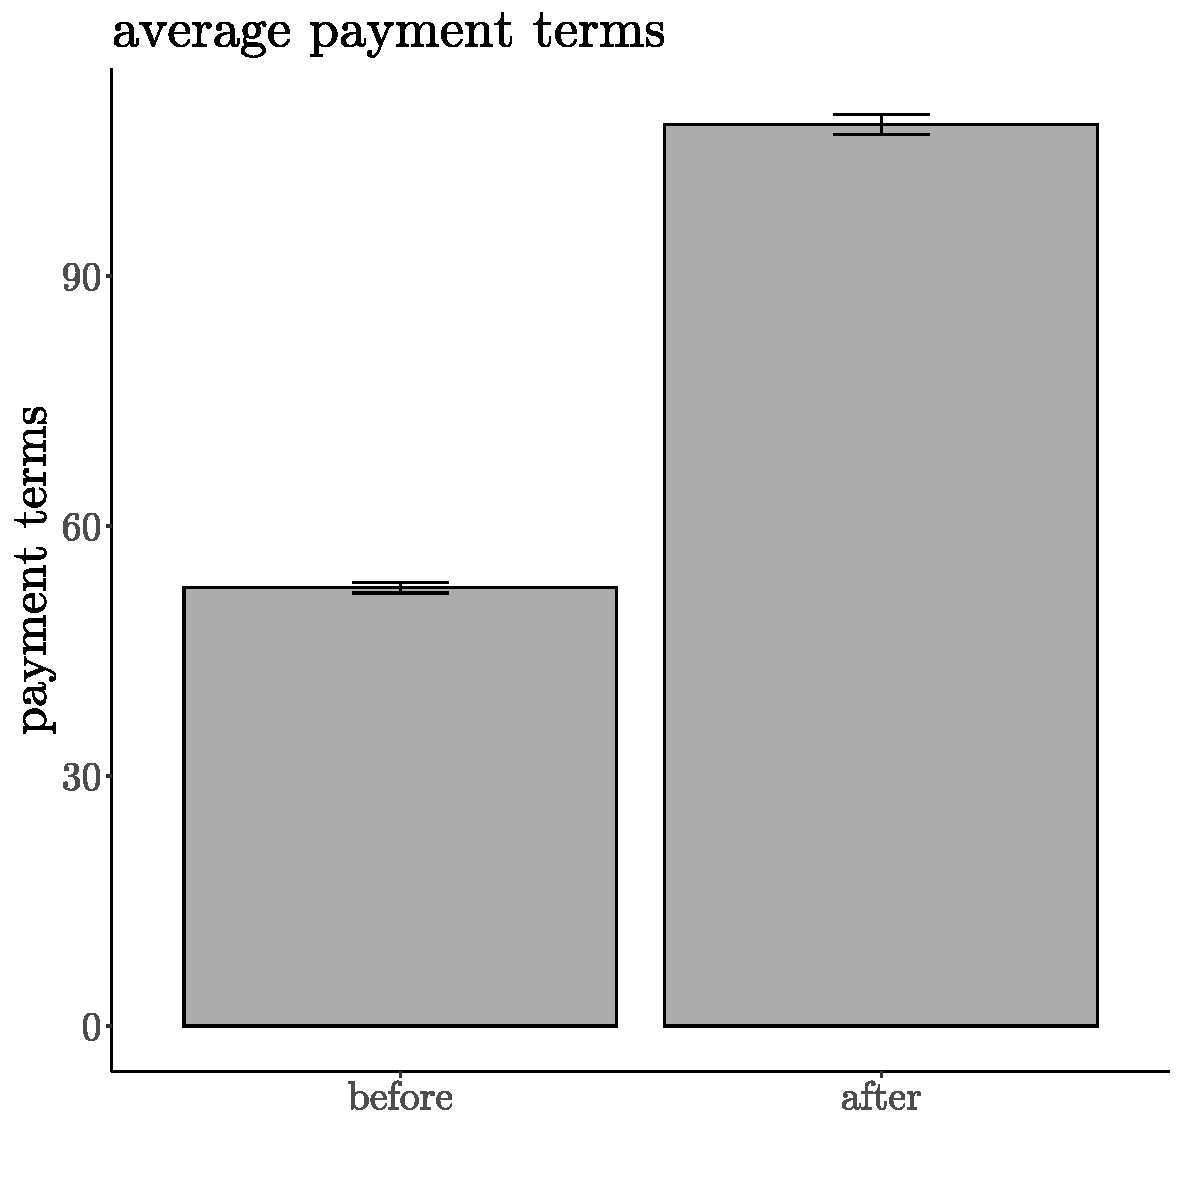
\includegraphics[width=\textwidth]{figures/bar.chart.payment.terms.pdf}
         \caption{$N=1,898$, all dyads. \vspace{24pt}}
         \label{fig:bar.pt}
     \end{subfigure}\hfill
     \begin{subfigure}[b]{0.47\textwidth}
        \centering
        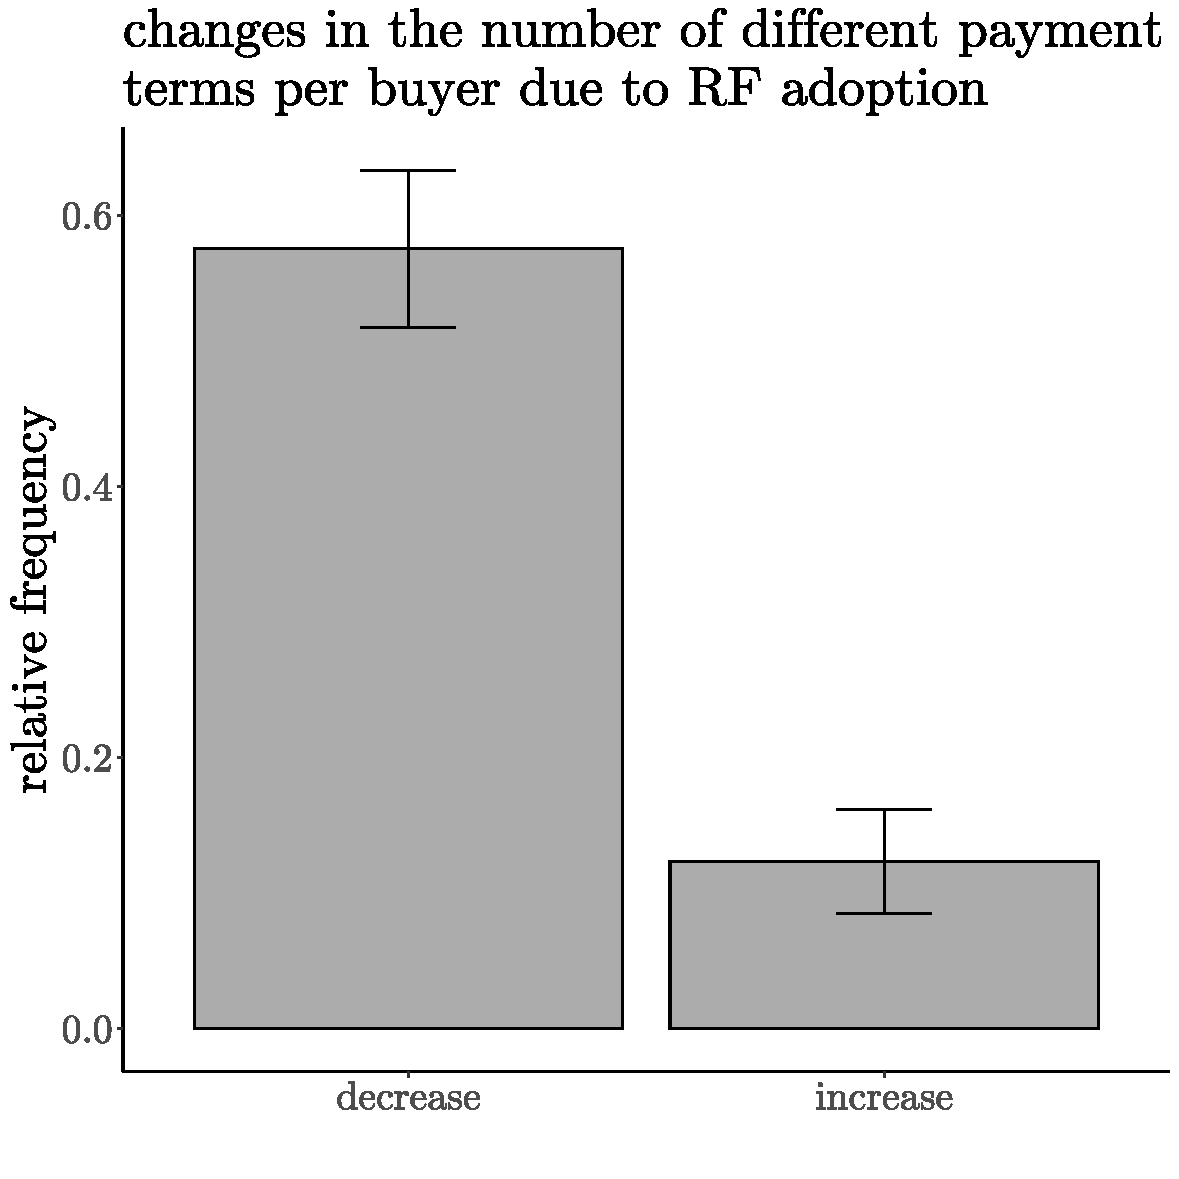
\includegraphics[width=\textwidth]{figures/bar.chart.programs.pdf}
        \caption{$N=73$, all buyers. \vspace{24pt}}
         \label{fig:bar.harmonize}
     \end{subfigure}     
    \caption{Bars indicate sample means, whiskers indicate standard errors. }
    \label{fig:bars}
\end{figure}


Turning to Hypotheses~2-5,  Model (1) in Table~\ref{tab:main:models} provides a fixed-effect regression model with payment term extension as the dependent variable and all control variables. Model (2) of the same table adds the variable \textit{initial payment terms}. Adding this variable increases the $R^2$ value from 6.1\% to 24.7\%, which is significant $(F=431, df1=1, df2=1,791, p<0.001$) and substantial: the variable \textit{initial payment terms} explains about 18.6\% of the variance in our sample's payment term extensions. In column (3), we add the variables \textit{mode}, \textit{standard terms}, and \textit{buyer experience}, leading to a significantly better model fit ($R^2=29.4\%, F=43.2, df1=3, df2=1,788, p<0.001$). The interaction of \textit{initial payment terms} and \textit{mode} in Model~(4) further increases the model fit ($R^2=29.7\%, F=6.62, df1=1, df2=1,787, p<0.05$). We will next interpret the results in Model (4), noting that they are consistent across all models. 


\begin{table}[htb]
{
\begin{center}
\scalebox{0.9}{
\begin{tabular}{%
l*{4}{cS[table-format=-3.3,table-space-text-post=***]}
}\toprule
&& \suc{(1)}&& \suc{(2)}&& \suc{(3)}&& \suc{(4)}\\\cline{3-3}\cline{5-5}\cline{7-7}\cline{9-9}\\[-9pt]
year &&\suc{(included)}&&\suc{(included)}&&\suc{(included)}&&\suc{(included)}\\
supplier industry &&\suc{(included)}&&\suc{(included)}&&\suc{(included)}&&\suc{(included)}\\
supplier country &&\suc{(included)}&&\suc{(included)}&&\suc{(included)}&&\suc{(included)}\\[5pt]
RF interest rate&&1.317&&-0.176&&0.954&&1.190\\
&&\suc{(2.330)}&&\suc{(2.551)}&&\suc{(1.958)}&&\suc{(1.964)}\\risk free rate&&3.246&&10.363&&12.717&&12.550\\
&&\suc{(8.972)}&&\suc{(9.887)}&&\suc{(10.298)}&&\suc{(10.141)}\\annual spend&&1.427&&0.752&&2.395&&2.453\\
&&\suc{(2.506)}&&\suc{(2.344)}&&\suc{(2.139)}&&\suc{(2.203)}\\supplier revenue&&-0.096&&-0.129&&0.621&&0.542\\
&&\suc{(1.387)}&&\suc{(1.518)}&&\suc{(1.369)}&&\suc{(1.386)}\\initial payment terms&&&&-0.902$^{***}$&&-0.891$^{***}$&&-0.880$^{***}$\\
&&\suc{}&&\suc{(0.046)}&&\suc{(0.036)}&&\suc{(0.037)}\\mode (1=manual)&&&&&&-16.113$^{***}$&&-15.549$^{***}$\\
&&\suc{}&&\suc{}&&\suc{(3.633)}&&\suc{(3.632)}\\standard term (1=yes)&&&&&&-20.529$^{***}$&&-20.661$^{***}$\\
&&\suc{}&&\suc{}&&\suc{(6.194)}&&\suc{(6.173)}\\buyer experience&&&&&&8.154$^{**}$&&8.564$^{**}$\\
&&\suc{}&&\suc{}&&\suc{(2.838)}&&\suc{(2.726)}\\initial payment terms × mode &&&&&&&&0.311$^{***}$\\
&&\suc{}&&\suc{}&&\suc{}&&\suc{(0.089)}\\\midrule
$N$&&\suc{1898}&&\suc{1898}&&\suc{1898}&&\suc{1898}\\
$R^2$&&0.06&&0.24&&0.29&&0.3\\
model&&\suc{fixed effects}&&\suc{fixed effects}&&\suc{fixed effects}&&\suc{fixed effects}\\\bottomrule
\multicolumn{9}{L{1.05\textwidth}}{\footnotesize\textit{Note. Payment term extensions are not standardized; initial payment terms are mean-centered but not scaled. All other continuous variables are standardized. The year factor variable, supplier industry, and supplier country are included in the regression models but not displayed here for brevity; robust standard errors are in parentheses, \pDefSig.}}
\end{tabular}%
}%scalebox
\end{center}
}
\caption{Fixed-effect regression on payment term extensions. }
\label{tab:main:models}
\end{table}%{htb} 

\textit{Initial payment terms} have a significant and substantial negative effect of -0.88 $(p<0.001)$, supporting Hypothesis~\ref{H:d0.neg} and rejecting Hypothesis~\ref{H:d0.pos}. Since neither the dependent variable (\textit{payment term extensions}) nor the independent variable (\textit{initial payment terms}) is scaled, this implies that, on average, for one day more initial payment terms, the average extension is about 0.88 days less. If this coefficient were -1 instead of -0.88, we would see perfect standardization. Suppliers that use RF manually bargain for an average of 15.55 days less payment term extensions ($p<0.001$), supporting Hypothesis~\ref{H:mode:direct}. Consistent with Hypothesis~\ref{H:mode:interact}, we find that for those suppliers, initial payment terms have a more positive impact on the extension ($\beta_{9}=0.31,p<0.001$), though their overall impact is still negative. Hypothesis~\ref{H:standardization} is also supported: buyers appear to be willing to forego an average of 20.66 days in payment terms when this leads to their standard terms ($p<0.001$). Hypothesis~\ref{H:experience} finds support: For one standard deviation more buyer experience, they manage to bargain about 8.6 additional days ($p<0.01$). 

Finally, turning to Hypothesis~6, we find support for~\ref{H:reduceTerms} $\big(t=4.68,\,df=72,$ $p<0.001; V=1,204.5,\,p<0.001\big)$, indicating that buyers indeed, on average, reduce the number of different payment terms. An additional test of proportions shows that a reduction of the number of payment terms occurs more often than an increase $\big(57.3\% \text{ vs. } 12.3\%; \chi^2=30.86,\,df=1,$ $p<0.001\big)$; Figure~\ref{fig:bar.harmonize} illustrates this test. In addition, we find that the coefficient of variation of RF payment terms (0.31) is significantly smaller than the coefficient of variation of initial payment terms (0.41), both measured on the buyer level  $\big(t=2.979,\,df=65,$ $p<0.01; V=1,392,\,p<0.01\big)$. The coefficient of variation of RF payment terms is still significantly different from 0 $\big(t=11.23,\,df=65,$ $p<0.001; V=1,770,\,p<0.001\big)$. Both findings suggest that buyers harmonize payment terms but not perfectly so. Table~\ref{tab:probit} reports the probit model estimates, where Model~(1) includes only control variables and Model~(2) also includes the hypothesized effect variable. The smaller AIC of the Model~(2) suggests an increase in model fit. Further, the variable \textit{RF program size} is significant ($p<0.05$), indicating that the number of different payment terms reduces more likely in larger programs, lending support to Hypothesis~\ref{H:salience}.


\begin{table}[htb]
{
\begin{center}
\scalebox{1}{
\begin{tabular}{%
l*{4}{cS[table-format=-3.3,table-space-text-post=***]}
}\toprule
&& \suc{(1)}&& \suc{(2)}\\\cline{3-3}\cline{5-5}\\[-9pt]
buyer industry \phantom{buyer industry}&&\suc{(included)}&&\suc{(included)}\\
buyer country &&\suc{(included)}&&\suc{(included)}\\[5pt]
buyer revenue&&0.592&&-0.105\\
&&\suc{(0.609)}&&\suc{(0.527)}\\buyer costs of goods sold&&-0.257&&0.173\\
&&\suc{(0.535)}&&\suc{(0.498)}\\RF program size&&&&1.162$^{*}$\\
&&\suc{}&&\suc{(0.542)}\\\midrule
$N$&&\suc{73}&&\suc{73}\\
AIC&&\suc{98.72}&&\suc{85.57}\\
model&&\suc{probit}&&\suc{probit}\\\bottomrule
\multicolumn{5}{L{0.75\textwidth}}{\footnotesize\textit{Note.  Dependent variable standardization = true indicates that a buyer reduced the number of different terms through the RF adoption. The buyer industry and buyer country variables are included in the models but not displayed here for brevity; robust standard errors are in parentheses, \pDefSig.}}
\end{tabular}%
}%scalebox
\end{center}
}
\caption{Probit regression on standardization.}
\label{tab:probit}
\end{table}%{htb} 

\subsection{Robustness checks}
\label{sec:robust}
Although we do not seek to imply causality, we carried out a series of tests to examine whether endogeneity unduly affects the results. The most critical finding of our analysis is the negative impact of initial payment terms on their extension. This suggests that the fairness and standardization motives are stronger than the financing cost motive; a somewhat surprising result. Still, there is a potential alternative explanation for this finding, which we will rule out next. It is conceivable that suppliers on short initial payment terms are on short terms because of unobserved factors, such as their credit rating or strategic importance. It might then be the case that the buyer uses RF to harmonize terms, particularly with those suppliers. To address this issue, we use an instrumental variable approach. To obtain an exogenous instrument, we consider the average payment terms of suppliers in this supplier's country (excluding the focal supplier) for each supplier. There is a high correlation among payment terms within each country, and by excluding the supplier, this measure is exogenous. We report the first step of this approach in Model~(1) of Table~\ref{tab:robust_1}. The significant coefficient of .96 ($p<0.001$) of \textit{average payment terms (supplier country)} suggests that this instrument is relevant. Model~(2) reports the IV model, finding significant support for Hypothesis~\ref{H:d0.neg} ($p<0.001$). Models~(3) and (4) report a similar IV approach considering the average payment terms of the supplier's industry as an instrument; this approach leads likewise to support of Hypothesis~\ref{H:d0.neg} ($p<0.001$). 

A selection bias might be driving some results. Based on several discussions with the RF provider and firm managers who use the RF provider's platform, we learned that most suppliers eventually implement RF. However, we further collected data on $N=96$ cases where suppliers eventually refused the adoption. Since this number is comparably small, we consider the corresponding Heckman selection model rather exploratory. Model~(5) in Table~\ref{tab:robust_1} shows the probit model as step~1 of the Heckman-selection model and Model~(6) the step~2 results. Again, \textit{initial payment terms} continue to impact \textit{payment term extensions} negatively, and other results continue to be consistent with our hypotheses. 

\begin{table}[htb]
{
\begin{center}
\scalebox{0.7}{
\begin{tabular}{%
l*{6}{cS[table-format=-3.3,table-space-text-post=***]}
}\toprule
&& \suc{1}&& \suc{2}&& \suc{3}&& \suc{4}&& \suc{5}&& \suc{6}\\\cline{3-3}\cline{5-5}\cline{7-7}\cline{9-9}\cline{11-11}\cline{13-13}
&& \suc{IV-country}&& \suc{IV-country}&& \suc{IV-ind}&& \suc{IV-ind}&& \suc{Heckman}&& \suc{Heckman}\\
&& \suc{step 1}&& \suc{step 2}&& \suc{step 1}&& \suc{step 2}&& \suc{step 1}&& \suc{step 2}\\[5pt]
year &&\suc{(included)}&&\suc{(included)}&&\suc{(included)}&&\suc{(included)}&&\suc{(included)}&&\suc{(included)}\\
supplier industry &&\suc{(included)}&&\suc{(included)}&&\suc{(included)}&&\suc{(included)}&&\suc{(included)}&&\suc{(included)}\\
supply country &&\suc{(included)}&&\suc{(included)}&&\suc{(included)}&&\suc{(included)}&&\suc{(included)}&&\suc{(included)}\\[5pt]
average payment terms&&0.958$^{***}$&&&&&&&&&&\\
 (supplier country)&&\suc{(0.064)}&&\suc{}&&\suc{}&&\suc{}&&\suc{}&&\suc{}\\average payment terms &&&&&&0.743$^{***}$&&&&&&\\
(supplier industry)&&\suc{}&&\suc{}&&\suc{(0.160)}&&\suc{}&&\suc{}&&\suc{}\\RF interest rate&&&&1.225&&&&0.809&&0.219$^{*}$&&3.189\\
&&\suc{}&&\suc{(1.903)}&&\suc{}&&\suc{(2.110)}&&\suc{(0.110)}&&\suc{(3.081)}\\risk free rate&&&&11.412&&&&13.420&&&&13.189$^{+}$\\
&&\suc{}&&\suc{(10.386)}&&\suc{}&&\suc{(10.118)}&&\suc{}&&\suc{(6.738)}\\annual spend&&&&2.524&&&&2.325&&0.137$^{*}$&&4.130\\
&&\suc{}&&\suc{(2.152)}&&\suc{}&&\suc{(2.197)}&&\suc{(0.067)}&&\suc{(2.549)}\\supplier revenue&&&&0.630&&&&0.616&&&&-0.498\\
&&\suc{}&&\suc{(1.271)}&&\suc{}&&\suc{(1.431)}&&\suc{}&&\suc{(1.510)}\\initial payment terms&&&&-0.733$^{***}$&&&&-0.976$^{***}$&&-0.048&&-0.914$^{***}$\\
&&\suc{}&&\suc{(0.121)}&&\suc{}&&\suc{(0.167)}&&\suc{(0.053)}&&\suc{(0.048)}\\mode (1=manual)&&&&-16.667$^{***}$&&&&-15.815$^{***}$&&&&-15.468$^{***}$\\
&&\suc{}&&\suc{(3.707)}&&\suc{}&&\suc{(3.595)}&&\suc{}&&\suc{(3.029)}\\standard term (1=yes)&&&&-20.776$^{***}$&&&&-20.396$^{**}$&&&&-20.808$^{***}$\\
&&\suc{}&&\suc{(6.170)}&&\suc{}&&\suc{(6.201)}&&\suc{}&&\suc{(2.133)}\\buyer experience&&&&7.025$^{*}$&&&&8.762$^{**}$&&&&7.966$^{**}$\\
&&\suc{}&&\suc{(2.805)}&&\suc{}&&\suc{(3.290)}&&\suc{}&&\suc{(2.837)}\\\midrule
$N$&&\suc{1898}&&\suc{1898}&&\suc{1898}&&\suc{1898}&&\suc{1994}&&\suc{1994}\\
model&&\suc{fixed effects}&&\suc{fixed effects}&&\suc{fixed Effects}&&\suc{fixed effects}&&\suc{Probit}&&\suc{fixed effects}\\
$R^2$&&0.1&&0.29&&0.01&&0.29&&&&0.46\\
AIC&&&&&&&&&&\suc{767.27}&&\\
\bottomrule
\multicolumn{13}{L{1.3\textwidth}}{\footnotesize\textit{Note. Payment term extensions are not standardized; initial payment terms are mean-centered but not scaled. All other continuous variables are standardized. The year factor variable, supplier industry, and supplier country are included in the regression models but not displayed here for brevity; (robust) standard errors are in parentheses, \pDefSig.}}
\end{tabular}%
}%scalebox
\end{center}
}
\caption{Robustness tests. Models (1)--(4) are instrumental variable models, and Models (5) and (6) relate to Heckman selection. }
\label{tab:robust_1}
\end{table}%{htb} 


Our data features a panel with approximately ten years of data. Although it does not state payment terms variation except for the time at which RF is introduced, it still allows us to run a difference-in-difference model. With this approach, we seek further support that firms on above-average payment terms (\textit{treatment} = 1) face a more minor payment terms extension. We consider the variable \textit{after} to indicate that a supplier has adopted RF. Table~\ref{tab:did} displays the estimates using a typical difference-in-difference specification. As seen in Model~(3), there is a negative interaction of \textit{adopted} and \textit{treatment} ($p<0.001$), which indicates that suppliers with initial payment terms above their buyer's average faced, on average, 49.5 days shorter extensions. 



\begin{table}[htb]
{
\begin{center}
\scalebox{1}{
\begin{tabular}{%
l*{4}{cS[table-format=-3.3,table-space-text-post=***]}
}\toprule
&& \suc{(1)}&& \suc{(2)}&& \suc{(3)}\\\cline{3-3}\cline{5-5}\cline{7-7}\\[-9pt]
supplier industry &&\suc{(included)}&&\suc{(included)}&&\suc{(included)}\\
supplier country &&\suc{(included)}&&\suc{(included)}&&\suc{(included)}\\[5pt]
RF interest rate&&1.598&&2.695$^{***}$&&1.899$^{*}$\\
&&\suc{(0.973)}&&\suc{(0.796)}&&\suc{(0.740)}\\risk free rate&&-1.805$^{**}$&&8.393$^{***}$&&7.648$^{***}$\\
&&\suc{(0.691)}&&\suc{(0.615)}&&\suc{(0.577)}\\annual spend&&1.134&&2.147$^{**}$&&1.649$^{*}$\\
&&\suc{(0.916)}&&\suc{(0.791)}&&\suc{(0.745)}\\supplier revenue&&0.469&&-0.499&&-0.891\\
&&\suc{(0.704)}&&\suc{(0.597)}&&\suc{(0.586)}\\mode (1=manual)&&-6.178$^{***}$&&-7.663$^{***}$&&-6.946$^{***}$\\
&&\suc{(1.677)}&&\suc{(1.358)}&&\suc{(1.306)}\\standard term (1=yes)&&-8.187$^{***}$&&-7.591$^{***}$&&-9.104$^{***}$\\
&&\suc{(1.439)}&&\suc{(1.243)}&&\suc{(1.241)}\\buyer experience&&0.003&&1.243$^{+}$&&1.681$^{**}$\\
&&\suc{(0.762)}&&\suc{(0.654)}&&\suc{(0.645)}\\after&&&&55.394$^{***}$&&78.447$^{***}$\\
&&\suc{}&&\suc{(1.392)}&&\suc{(2.040)}\\treatment&&&&25.318$^{***}$&&50.468$^{***}$\\
&&\suc{}&&\suc{(1.063)}&&\suc{(1.119)}\\after × treatment&&&&&&-49.470$^{***}$\\
&&\suc{}&&\suc{}&&\suc{(2.534)}\\\midrule
$N$ (suppliers) &&\suc{1898}&&\suc{1898}&&\suc{1898}\\
$R^2$&&0.26&&0.46&&0.54\\
model&&\suc{random effects}&&\suc{random effects}&&\suc{random effects}\\\bottomrule
\multicolumn{7}{L{0.9\textwidth}}{\footnotesize\textit{Note. After = 1 indicates that the supplier has adopted RF; treatment = 1 indicates that the supplier's initial payment terms are above the buyer's average payment terms with other suppliers. The year factor variable, supplier industry, and supplier country are included in the regression models but not displayed here for brevity. Robust standard errors are in parentheses, \pDefSig.}}
\end{tabular}%
}%scalebox
\end{center}
}
\caption{Robustness checks, difference-in-difference specifications with random effects on the supplier level and dependent variable payment terms. }
\label{tab:did}
\end{table}%{htb} 

We finally report two further robustness checks in Table~\ref{tab:robust_2}. Models~(1) and (2) report panel models with buyer-level random effects and buyer industry and country controls. Both models feature results consistent with our fixed-effect-model-based primary analysis. Comparing the random-effects models with their fixed-effect counterparts, a Hausman test suggests that (1) is unaffected by endogeneity ($\chi^2=37.13,\,df=37,\,p=0.46$) whereas (2) is likely affected ($\chi^2=876.1,\,df=38,\,p<0.001$). Although the coefficients are consistent across all models, we posit that fixed effects appear more appropriate in our setting. As mentioned above, a large part of this study's data is identical to a former study on RF adoption \citep{Wuttke2019}. Models~(3) and (4) of Table~\ref{tab:robust_2} restrict the dataset to exactly those supplier-buyer dyads that \citet{Wuttke2019} analyzes and find that this subset of 1,403 observations leads to consistent results.

\begin{table}[htb]
{
\begin{center}
\scalebox{0.86}{
\begin{tabular}{%
l*{4}{cS[table-format=-3.3,table-space-text-post=***]}
}\toprule
&& \suc{(1)}&& \suc{(2)}&& \suc{(3)}&& \suc{(4)}\\\cline{3-3}\cline{5-5}\cline{7-7}\cline{9-9}\\[-9pt]
year &&\suc{(included)}&&\suc{(included)}&&\suc{(included)}&&\suc{(included)}\\
supplier industry &&\suc{(included)}&&\suc{(included)}&&\suc{(included)}&&\suc{(included)}\\
supplier country &&\suc{(included)}&&\suc{(included)}&&\suc{(included)}&&\suc{(included)}\\
buyer industry &&\suc{(included)}&&\suc{(included)}\\
buyer country &&\suc{(included)}&&\suc{(included)}\\[5pt]RF interest rate&&0.713&&0.998&&2.087&&2.449\\
&&\suc{(2.062)}&&\suc{(2.054)}&&\suc{(1.559)}&&\suc{(1.500)}\\risk free rate&&13.354&&13.236&&26.651$^{*}$&&26.081$^{*}$\\
&&\suc{(10.240)}&&\suc{(10.068)}&&\suc{(11.510)}&&\suc{(11.107)}\\annual spend&&2.526&&2.631&&3.782&&3.928\\
&&\suc{(2.124)}&&\suc{(2.197)}&&\suc{(2.362)}&&\suc{(2.428)}\\supplier revenue&&0.671&&0.609&&-0.547&&-0.676\\
&&\suc{(1.374)}&&\suc{(1.401)}&&\suc{(1.243)}&&\suc{(1.225)}\\initial payment terms&&-0.886$^{***}$&&-0.873$^{***}$&&-0.888$^{***}$&&-0.877$^{***}$\\
&&\suc{(0.036)}&&\suc{(0.037)}&&\suc{(0.047)}&&\suc{(0.053)}\\mode (1=manual)&&-16.491$^{***}$&&-15.909$^{***}$&&-10.012$^{***}$&&-9.699$^{***}$\\
&&\suc{(3.654)}&&\suc{(3.683)}&&\suc{(2.567)}&&\suc{(2.342)}\\standard term (1=yes)&&-21.367$^{***}$&&-21.605$^{***}$&&-23.012$^{***}$&&-23.127$^{***}$\\
&&\suc{(6.237)}&&\suc{(6.233)}&&\suc{(5.890)}&&\suc{(5.826)}\\buyer experience&&5.441$^{**}$&&5.485$^{**}$&&5.989$^{*}$&&6.788$^{**}$\\
&&\suc{(1.851)}&&\suc{(1.778)}&&\suc{(2.506)}&&\suc{(2.447)}\\initial payment terms × mode&&&&0.332$^{***}$&&&&0.452$^{***}$\\
&&\suc{}&&\suc{(0.095)}&&\suc{}&&\suc{(0.082)}\\\midrule
$N$&&\suc{1898}&&\suc{1898}&&\suc{1403}&&\suc{1403}\\
$R^2$&&0.36&&0.37&&0.31&&0.32\\
model&&\suc{random effects}&&\suc{random effects}&&\suc{fixed effects}&&\suc{fixed effects}\\\bottomrule
\multicolumn{9}{L{1.13\textwidth}}{\footnotesize\textit{Note. Payment term extensions are not standardized; initial payment terms are mean-centered but not scaled. All other continuous variables are standardized. The year factor variable, supplier industry, and supplier country are included in the regression models but not displayed here for brevity; buyer country and industry are likewise included in (1) and (2); robust standard errors are in parentheses,\pDefSig.}}
\end{tabular}%
}%scalebox
\end{center}
}
\caption{Robustness checks. Models (1) and (2) feature random effects. Models (3) and (4) are performed on a subset matching the formerly published study \citet{Wuttke2019}.}
\label{tab:robust_2}
\end{table}%{htb} 



\FloatBarrier

\section{Discussion and conclusion}
Our study's key research question is how firms extend payment terms in the context of RF adoption. Our game-theoretical model features three motives and predicts how, if applicable, they would shape bargaining outcomes in industry. We then derived six hypotheses, which we tested in reduced form. Except for a competing hypothesis, we find support for all.

So, are all motives present?

The rejection of Hypothesis~\ref{H:d0.pos} suggests that the financing cost motive is far less salient than expected. After all, buying firms mainly introduce RF to improve payment terms, and Hypothesis~\ref{H:d0.pos} is fairly consistent with extant models \citep[e.g.,][]{Lekkakos2016, Kouvelis2020,vanderVliet2015, Wuttke2016}, so we would have expected longer payment term extensions for suppliers with longer initial payment terms; but this is not reflected in our sample. Still, Hypothesis~\ref{H:mode:interact} suggests that at least suppliers that use a more sophisticated approach to RF seem to emphasize financing cost effects more. So, in part, firms do account for the financing cost motive, but clearly less than expected. We explain this observation as the financing rates under RF tend to be so favorable that one day more or less hardly makes a difference: for a buyer and supplier with an annual spend of \$1,000,000 and an annual RF interest of 2\%, an additional payment term day corresponds to \$55. Even extending payment terms by a relatively considerable amount of 20 days more or less translates to only \$1,100, about 0.1\% of the annual spend. To put this into perspective, when suppliers offer discounts to stimulate more demand, that requires perhaps 5\%-10\% to be effective. Therefore, the financing costs and, some more or fewer days, objectively, hardly matter. But when the financing costs are fairly insensitive to even larger changes in the bargaining solution, we argue that firms build their idea of what is a good outcome for them on other factors, too.

Support for Hypotheses~\ref{H:d0.neg},~\ref{H:reduceTerms}, and~\ref{H:salience} suggests the existence of the fairness motive. Accordingly, payment terms are not extended by more if they are already long, but by less---suppliers with long payment terms would find it unfair to extend them even more. Likewise, payment terms are extended by more for suppliers on shorter terms---buyers would find it unfair not to achieve an outcome comparable to other suppliers, given all suppliers obtain similar financing conditions with RF. In some cases, our model predicts perfect standardization of payment terms, and indeed, the estimates in our model are fairly close. One might object that the very pattern of standardizing payment terms could also result from the standardization motive. However, our models include the variable \textit{standard term}, which captures whether the RF payment terms are most frequently used. In our sample, this happens in about 59\% of the negotiations. The significant negative impact of this variable indicates that buyers are willing to forego about 20 days in payment terms when this leads to standardized terms. If only the standardization motive drove the significance of Hypothesis~\ref{H:d0.neg}, then the coefficient of initial payment terms should not be negative when controlling for \textit{standard term}. Vice-versa, if the standardization were entirely driven by the fairness motive (which is a feasible outcome according to Proposition~\ref{prop:fairness}), we would not expect to see the support for Hypothesis~\ref{H:standardization}; the fairness motive does not, in general, favor a negative impact of standardization. Therefore, we conclude that both the fairness and the standardization motive are present. Together, they lead to a \textit{harmonization of payment terms}; with this concept, we capture that payment terms across suppliers either get perfectly standardized or at least the relative differences decrease. 

Turning to managerial implications, we cannot say whether harmonization is optimal, as witnessed in our dataset. However, buying firm managers who ignore this facet seem to be ill-advised when crafting an RF and payment terms strategy. They are likely miscalculating their expected benefits. At the same time, managers who only focus on harmonization might be underperforming as they deviate from profit-maximizing behavior, downplaying the financing cost motive. A careful assessment based on the buyer's supply chain strategy can help. Our study also has implications for RF providers who often consult with (potential) clients before starting an RF program. Our results should be reflected in their work, and they should carefully differentiate between the potential impact on days payables outstanding (which is one of their top-sales arguments) and supply chain impact (which requires a deeper understanding of harmonization). Simple calculators might be misleading, whereas the emphasis on fairness and standardization aspects is valuable.

Finally, as with all econometric studies, ours has some limitations. While we carefully address a series of potential endogeneity issues, it is always difficult to establish causality with secondary data. If future research could address two shortcomings, it would be valuable to treat selection biases thoroughly. Although we estimated a selection model, we only had information on 96 suppliers who declined an offer. Further selection biases can arise when RF providers select not to offer RF programs to some buyers or buyers decide not to offer RF to some suppliers. Since all buyers and suppliers in our dataset use RF from the same RF provider, we cannot rule out idiosyncracies, and it is conceivable that buyers and suppliers might behave differently in other programs. Data from other RF providers could help to explore this. Another aspect is the lack of causality of our tests. Our secondary dataset neither features fairness-related measures ($\beta$ and $\gamma$ in our model) nor the value of standardization ($\lambda$ in our model). As obtaining those variables through any secondary data approach will be very difficult, a controlled field experiment could shed more light on the causal effects. Nevertheless, our study represents the first foray into predicting and explaining payment term extensions in the RF context. 


\def\enoteformat{\rightskip=0pt \leftskip=0pt \parindent=0em
  \leavevmode\llap{\makeenmark}}


\singlespacing
\begin{flushleft}
\setlength{\bibsep}{0pt plus 0.3ex}
\bibliographystyle{agsm} % outcomment this and next line in Case 1
\bibliography{literature} % if more than one, comma separated
\footnotesize
\theendnotes
\end{flushleft}

\begin{appendices}
\onehalfspacing
\section{Proofs}
\normalsize

\begin{proof}{Proposition~\ref{prop:hyper}.} Define the objective function in Eq~(\ref{eq:obj}) as 
\begin{equation}\label{eq:K:gen}
    K\left(d_r\right) := 
\left(
U_{b,r}\left(d_r\right) - U_{b,0}\left(d_0\right)
\right)^\alpha
\left(
U_{s,r}\left(d_r\right) - U_{s,0}\left(d_0\right)
\right)^{\left(1-\alpha\right)}.
\end{equation}
Inserting utility functions~(\ref{eq:utilities}) and $\beta=\gamma=\lambda=0$ yields
$K(d_r)=(d_r i_b-d_0 i_b)^{\alpha } (d_0 i_s-d_r i_r)^{1-\alpha }.$ Since the logarithm is a strictly monotone function and $K\left(d_r\right)>0$ for the optimal solution, we can also maximize $\log\left(K\left(d_r\right)\right)$. Since all functions are smooth, consider $\frac{\partial }{\partial d_r}\log\left(K\left(d_r\right)\right)=\frac{-(1-\alpha) d_0 i_r-\alpha  d_0 i_s+d_r i_r}{(d_0-d_r) (d_0 i_s-d_r i_r)}\equalD 0$, yielding  $\dHyp := \left(1+\frac{i_s-i_r}{i_r}\alpha\right)d_0$. To show optimality, consider $\frac{\partial^2 }{\partial d_r^2}\log\left(K\left(d_r\right)\right)=\frac{\alpha  d_0 (i_r-i_s) (d_0 (i_r+i_s)-2 d_r i_r)-i_r^2 (d_0-d_r)^2}{(d_0-d_r)^2 (d_r i_r-d_0 i_s)^2}$. Then $\frac{\partial^2 }{\partial d_r^2}\log\left(K\left(\dHyp\right)\right)=
-\frac{i_r^2}{d_0^2 (i_s - i_r)^2 (1- \alpha) \alpha} <0$ proving optimality.
\end{proof}



\begin{proof}{Proposition~\ref{prop:fairness}.}
Suppose $\beta>0, \gamma>0$ and $\lambda=0$. Define 
\begin{equation}\label{eq:k}
    \begin{aligned}
k_1\left(d_r\right) := &    \left(
i_bd_r - \beta \left(\dref-d_r\right) - i_bd_0
\right)^\alpha
\left(
-i_rd_r  +i_sd_0
\right)^{\left(1-\alpha\right)}\\
k_2\left(d_r\right) :=& \left(
i_b\dref- i_bd_0
\right)^\alpha
\left(
-i_r\dref +i_sd_0
\right)^{\left(1-\alpha\right)} \text{, and}\\
k_3\left(d_r\right) :=& \left(
i_bd_r - i_bd_0
\right)^\alpha
\left(
-i_rd_r - \gamma \left(d_r-\dref\right)  + i_sd_0
\right)^{\left(1-\alpha\right)}
    \end{aligned}
\end{equation}
on the permissible domain $d_r\in\left\{d_r|K\left(d_r\right)>0\right\}$. Then $K\left(d_r\right)$ is a piece-wise differentiable function, except for at $d_r=\dref$, and we can write%
\begin{equation}\label{eq:K}
K\left(d_r\right) = \begin{cases}
k_1\left(d_r\right) & \text{ , if } d_r < \dref\\
k_2\left(d_r\right) & \text{ , if } d_r = \dref\\
k_3\left(d_r\right)& \text{ , if }  d_r > \dref
\end{cases}
\end{equation}
Let $d_i^* = \argmax_{d_r}\left\{k_i\left(d_r\right)\right\}$ for $i=1,2,3$.\newline
Solving $\frac{\partial k_1\left(d_r\right) }{\partial d_r}=\frac{d_0 i_b ((\alpha -1) i_r-\alpha  i_s)-\alpha  \beta  d_0 i_s+d_r i_r (\beta +i_b)+(\alpha -1) \beta  \dref i_r}{(d_r i_r-d_0 i_s) (-d_0 i_b+d_r (\beta +i_b)-\beta  \dref)}\equalD 0$ yields the unique candidate\newline
$d_1^* = \frac{d_0 i_b ((1-\alpha)  i_r+\alpha  i_s)+\alpha  \beta  d_0 i_s+(1-\alpha) \beta  \dref i_r}{i_r (\beta +i_b)}$. Evaluating the second derivative at $d_1^*$ leads to\newline
$-\frac{i_r^2 (\beta +i_b)^2}{(1-\alpha) \alpha  \left(d_0 i_b (i_r-i_s)-\beta  d_0 i_s+\beta  \dref i_r\right)^2}<0$. Therefore, $d_1^*$ is the unique maximum of $k_1$. Further, since $d_1^*$ is the only root of $\frac{\partial k_1\left(d_r\right) }{\partial d_r}$ and since $k_1$ is differentiable, $d_r<d_1^*\Rightarrow \frac{\partial k_1\left(d_r\right) }{\partial d_r}>0 $ and $d_r>d_1^*\Rightarrow \frac{\partial k_1\left(d_r\right) }{\partial d_r}<0$. Analog, we can determine $d_3^*=\alpha  d_0 \left(\frac{i_s}{\gamma +i_r}-1\right)+d_0+\frac{\alpha  \gamma  \dref}{\gamma +i_r}$ and establish that $d_r<d_3^*\Rightarrow \frac{\partial k_3\left(d_r\right) }{\partial d_r}>0$ and $d_r>d_3^*\Rightarrow \frac{\partial k_3\left(d_r\right) }{\partial d_r}<0.$

Suppose $d_1^*>\dref$ and $d_3^*<\dref$. Then, for all $d_r<\dref$, it holds that $k_1\left(d_r\right)<k_1\left(\dref\right)=k_2\left(\dref\right)$, which follows from comparing $k_1$ and $k_2$. Analog, $k_3\left(d_r\right)<k_3\left(\dref\right)=k_2\left(\dref\right)$. Therefore, $d_r=\dref$ maximizes $K\left(d_r\right)$. Suppose $d_1^*<\dref$ and $d_3^*<\dref$. Then $\dref$ dominates $d_3^*$. But since $k_2\left(\dref\right)=k_1\left(\dref\right)<k_1\left(d_1^*\right)$, $d_1^*$ maximizes $K\left(d_r\right)$. Suppose $d_1^*>\dref$ and $d_3^*>\dref$. Then $\dref$ dominates $d_1^*$. But since $k_2\left(\dref\right)=k_3\left(\dref\right)<k_3\left(d_3^*\right)$, $d_3^*$ maximizes $K\left(d_r\right)$. Moreover,  $d_1^*<\dref\Leftrightarrow d_0<\frac{ i_r (\alpha  \beta +i_b)}{i_b (\alpha (i_s- i_r)+i_r)+\alpha  \beta  i_s}\dref$ and  $d_3^*>\dref\Leftrightarrow d_0 >\frac{  \left(1-\alpha\right)\gamma  +i_r}{\left(1-\alpha\right)\gamma +\alpha \left(i_s- i_r\right)+i_r}\dref$. Further, it can be shown that $\frac{ i_r (\alpha  \beta +i_b)}{i_b (\alpha (i_s- i_r)+i_r)+\alpha  \beta  i_s}<\frac{  \left(1-\alpha\right)\gamma  +i_r}{\left(1-\alpha\right)\gamma +\alpha \left(i_s- i_r\right)+i_r}$ so that either $d_0<\frac{ i_r (\alpha  \beta +i_b)}{i_b (\alpha (i_s- i_r)+i_r)+\alpha  \beta  i_s}\dref$ or $d_0 >\frac{  \left(1-\alpha\right)\gamma  +i_r}{\left(1-\alpha\right)\gamma +\alpha \left(i_s- i_r\right)+i_r}\dref$ holds but not both. Expressing $d_1^*$ and $d_3^*$ in terms of $\dHyp$ completes the proof.
\end{proof}



\begin{proof}{Corollary~\ref{cor:pos.extensions}.}
Proof by contradiction. Suppose, $d^{f}_r - d_0 < 0$. Since $\lambda=0$, $ U_{b,r}\left(d_r^f\right)-U_{b,0}\left(d_0\right)<0$. In that case, the buyer would not offer RF.
\end{proof}

\begin{proof}{Corollary~\ref{cor:ptx.d0}.}
(i) Consider $d_r^f$ as defined in~(\ref{eq:drf}) and calculate $\frac{\partial}{\partial d_0}\left(d_r^f-d_0\right)$ for each case separately:
    \begin{equation}\label{eq:d.ext}
        \frac{\partial}{\partial d_0}\left(d_r^f-d_0\right)= \begin{cases}
        \frac{\alpha  i_s}{i_r}-\frac{\beta +\alpha  i_b}{\beta +i_b}
  & \text{, if } d_0 < \frac{ i_r (i_b + \alpha \beta)}{
  i_b (i_r + \left(i_s- i_r\right) \alpha) + i_s \alpha \beta)}\dref\\
  -1 & \text{, if }d_0\in\left[\frac{ i_r (i_b + \alpha \beta)}{
  i_b (i_r + \left(i_s- i_r\right) \alpha) + i_s \alpha \beta)}\dref,\frac{ i_r + \left(1- \alpha\right) \gamma}{i_r + (i_s-i_r) \alpha + (1-\alpha)\gamma}\dref\right]\\
  \alpha  \left(\frac{i_s}{\gamma +i_r}-1\right)& \text{, if } d_0 >\frac{ i_r + \left(1- \alpha\right) \gamma}{i_r + (i_s-i_r) \alpha + (1-\alpha)\gamma}\dref
        \end{cases}
    \end{equation}
To prove statement (a), for $d_0 < \frac{ i_r (i_b + \alpha \beta)}{
  i_b (i_r + \left(i_s- i_r\right) \alpha) + i_s \alpha \beta)}\dref$, this derivative becomes positive if and only if $\frac{\alpha  i_s}{i_r}-\frac{\beta +\alpha  i_b}{\beta +i_b}>0\Leftrightarrow i_s  >\frac{i_b \alpha + \beta}{i_b\alpha + \beta\alpha}i_r$. Turning to statement (b), for $d_0 >\frac{ i_r + \left(1- \alpha\right) \gamma}{i_r + (i_s-i_r) \alpha + (1-\alpha)\gamma}\dref$  this derivative becomes positive if $ i_s>i_r + \gamma$.
  
  Further, if either $d_0 < \frac{ i_r (i_b + \alpha \beta)}{
  i_b (i_r + \left(i_s- i_r\right) \alpha) + i_s \alpha \beta)}\dref$ and $i_s  <\frac{i_b \alpha + \beta}{i_b\alpha + \beta\alpha}i_r$,
  $d_0 >\frac{ i_r + \left(1- \alpha\right) \gamma}{i_r + (i_s-i_r) \alpha + (1-\alpha)\gamma}\dref$ and $ i_s<i_r + \gamma$, or 
 $ d_0\in\left[\frac{ i_r (i_b + \alpha \beta)}{
  i_b (i_r + \left(i_s- i_r\right) \alpha) + i_s \alpha \beta)}\dref,\frac{ i_r + \left(1- \alpha\right) \gamma}{i_r + (i_s-i_r) \alpha + (1-\alpha)\gamma}\dref\right]$, the derivative becomes negative.


Turning to (ii), (a) $\beta\rightarrow 0\Rightarrow \dHyp + \frac{(\dref-d_0) (1 - \alpha) \beta}{i_b + \beta}\rightarrow\dHyp$ and 
  $\gamma\rightarrow 0\Rightarrow \dHyp-\frac{(d_0 i_s-\dref i_r) \alpha \gamma}{i_r (i_r + \gamma)}\rightarrow\dHyp$. Therefore, for $\beta\rightarrow 0$ and $\gamma\rightarrow 0$ it holds that $d_r^f\rightarrow\dHyp$. (b) Consider the terms in Eq~(\ref{eq:d.ext}) and note  $$
  \lim_{\beta\rightarrow\infty,\gamma\rightarrow\infty}
        \left(\frac{\partial}{\partial d_0}\left(d_r^f-d_0\right)\right) = \begin{cases}
        -1+\frac{i_s}{i_r}\alpha
  & \text{, if } d_0 < \frac{ i_r }{i_s}\dref\\
  -1 & \text{, if }d_0\in\left[\frac{ i_r }{i_s}\dref,\dref\right]\\
-\alpha& \text{, if } d_0 >\dref.
        \end{cases}
  $$
  
\end{proof}

\begin{proof}{Corollary~\ref{cor:relative.fairness}.}
Statement (a) is true because $\frac{\partial^2}{\partial d_0\partial\beta}\left(d_r^f-d_0\right)=-\frac{(1-\alpha) i_b}{(\beta +i_b)^2}<0$ for $d_0 < \frac{ i_r (i_b + \alpha \beta)}{  i_b (i_r + \left(i_s- i_r\right) \alpha) + i_s \alpha \beta)}\dref$. Statement (b) is true because $\frac{\partial^2}{\partial d_0\partial\gamma}\left(d_r^f-d_0\right)= -\frac{\alpha  i_s}{(\gamma +i_r)^2}<0 $ for $ d_0 >\frac{ i_r + \left(1- \alpha\right) \gamma}{i_r + (i_s-i_r) \alpha + (1-\alpha)\gamma}\dref$.
\end{proof}

\begin{proof}{Proposition~\ref{prop:full}.}
Suppose, $\beta>0$, $\gamma>0$, and $\lambda>0$. Then, using the definition of $K$ in Eq~(\ref{eq:K:gen}), $K(\dref)=(-d_0 i_b+\dref i_b+\lambda )^{\alpha } (d_0 i_s-\dref i_r)^{1-\alpha }=:\kappa\left(\lambda\right)$ with $\kappa'\left(\lambda\right)=\alpha  (-d_0 i_b+\dref i_b+\lambda )^{\alpha -1} (d_0 i_s-\dref i_r)^{1-\alpha}$. Since $-d_0 i_b+\dref i_b>0$ and $d_0 i_s-\dref i_r>0$, there exists an $\varepsilon>0$ such that $\kappa'\left(\lambda\right)>\varepsilon$ for all $\lambda$. Therefore, $\lim_{\lambda\rightarrow\infty}\kappa\left(\lambda\right)=\infty$. Since there exists a bound, $\overline K$ such that $K(d_r)<\overline K$ for all $d_r\neq\dref$, there must be a range that we denote by $\left[\underline{d}\left(\lambda_0\right),\overline{d}\left(\lambda_0\right)\right]$ for sufficiently large $\lambda_0$ such that $K(\dref)>K(d_r)$ for $d_r\neq \dref$.
\end{proof}


\begin{proof}{Corollary~\ref{cor:standardization}.}
(i) Since $d_0\in\left[d\left(\lambda_0\right),\frac{ i_r (i_b + \alpha \beta)}{
  i_b (i_r + \left(i_s- i_r\right) \alpha) + i_s \alpha \beta)}\dref\right]\subset\left[\underline{d}\left(\lambda_0\right),\overline{d}\left(\lambda_0\right)\right]$ by definition, standardization benefits lead to payment terms $\dref$ whereas for $\lambda=0$ the bargaining outcome per Proposition~\ref{prop:fairness} is  $\dHyp + \frac{(\dref-d_0) (1 - \alpha) \beta}{i_b + \beta}<\dref$. Analog, we can prove (ii).
\end{proof}

\begin{proof}{Corollary~\ref{cor:alpha:limit}.}
Suppose $\beta=\gamma=0$ and suppose $\lambda=0$ then $\lim_{\alpha\rightarrow 1}d_r^h=\frac{i_s}{i_r}d_0$ such that $\lim_{\alpha\rightarrow 1}\left(d_0 i_s-d_r^h i_r\right)=0$. In other words, payment terms cannot become longer than $\frac{i_s}{i_r}d_0$ because otherwise, the supplier would not adopt RF, contradicting our implicit participation assumption. Following Corollary~\ref{cor:standardization}, if $\lambda>0$ is sufficiently large, $\dref<\frac{i_s}{i_r}d_0$ is the bargaining outcome. 
\end{proof}

\end{appendices}





%%%%%%%%%%%%%%%%%
\end{document}
%%%%%%%%%%%%%%%%%
